% -*- coding: utf-8 -*-
% Русский перевод: V. G. Baryshevsky,
% Rotation of particle spin in a storage ring with a polarized beam
% and measurement of the particle EDM, tensor polarizability and
% elastic zero-angle scattering amplitude,
% J. Phys. G: Nucl. Part. Phys. 35 (2008) 035102.
\documentclass[11pt,a4paper]{article}

\usepackage[margin=2.2cm]{geometry}
\usepackage{fontspec}
\usepackage{polyglossia}
\setdefaultlanguage{russian}
\setotherlanguage{english}
\setmainfont{Times New Roman}
\newfontfamily\cyrillicfont{Times New Roman}
\newfontfamily\cyrillicfonttt{Consolas}
\usepackage{amsmath,amssymb,mathtools}
\usepackage{graphicx}
\usepackage{float}
\usepackage{setspace}
\usepackage{microtype}
\usepackage[hidelinks]{hyperref}
\usepackage{xcolor}

\graphicspath{{./}}
\setstretch{1.12}
\allowdisplaybreaks
\DeclareMathOperator{\Tr}{Tr}
\DeclareMathOperator{\Reop}{Re}
\DeclareMathOperator{\Imop}{Im}

\newcommand{\hvec}[1]{\hat{\vec{#1}}}

\title{Вращение спина частицы в накопителе с поляризованным пучком}
\author{V. G. Baryshevsky}
\date{}

\begin{document}

\begin{center}
{\LARGE\bfseries Вращение спина частицы в накопителе с поляризованным пучком:\\
измерение ЭДМ, тензорной поляризуемости\\
и амплитуды упругого рассеяния на нулевой угол}\\[1.1em]
{\large V.~G.~Baryshevsky}\\[0.5em]
{\small Research Institute for Nuclear Problems, Belarus State University,\\
11 Bobruyskaya Str., Minsk 220050, Belarus}\\[0.3em]
{\small\texttt{bar@inp.minsk.by}}\\[0.7em]
{\small\textit{J.\ Phys.\ G: Nucl.\ Part.\ Phys.} \textbf{35} (2008) 035102}\\
{\small Получено 27 июня 2007; опубликовано 25 января 2008}
\end{center}

\begin{center}
{\small\textit{Русский перевод полного текста. Формулы сверены со сканом оригинала
и arXiv-исходником \texttt{hep-ph/0603191}.\\
Обозначения журнальной версии: спин --- $\vec{S}$; единичные векторы --- $\vec{e}$;
частота T-BMT --- $\vec{\Omega}$; ядерная прецессия --- $\vec{\Omega}_{\mathrm{nuc}}$.}}
\end{center}

\vspace{0.8em}
\noindent\textbf{Аннотация.}
Получены уравнения движения спина частицы в накопительном кольце с учётом
вкладов тензорных электрической и магнитной поляризуемостей частицы, а также
вращения спина и двулучепреломления в поляризованной внутренней мишени.
Исследование эффектов вращения спина и двулучепреломления для частицы
в накопителе высоких энергий позволяет измерить как спин-зависимую вещественную
часть амплитуды когерентного упругого рассеяния на нулевой угол, так и тензорные
электрическую (магнитную) поляризуемости.

\tableofcontents
\newpage

\section{Введение}

Исследование спин-зависимых взаимодействий элементарных частиц при высоких
энергиях --- важная часть программ научных исследований на накопителях~\cite{Lehar,Engels,Kacharava}.
Такие работы ведутся с поляризованными пучками и поляризованными мишенями.
Зависимость сечений рассеяния от спина частицы --- предмет многочисленных
исследований. Сейчас готовятся эксперименты по измерению спин-зависимой
части амплитуды рассеяния вперёд~\cite{Engels,Kacharava}.

В экспериментальной физике частиц хорошо известно, как измерять спин-зависимое
сечение. Однако измерение спин-зависимой части амплитуды рассеяния вперёд
остаётся сложной задачей.

Однозначный и прямой метод измерения вещественной части спин-зависимой
амплитуды рассеяния вперёд для частиц высоких энергий предложен
в~\cite{Bary83a,Bary83b,BaryDub89,BaryShekht96,Bary92,Bary93,Bary98,BarySTORI05}.
В частности, вещественную часть спин-зависимой амплитуды рассеяния вперёд
для протонов (дейтронов, антипротонов), проходящих через поляризованную
ядерную мишень, можно найти, измеряя вращение спина частицы. Эффект
двулучепреломления дейтрона (то есть явление вращения и осцилляций спина
дейтрона) позволяет измерить вещественную часть спин-зависимой амплитуды
рассеяния вперёд для дейтронов, проходящих через неполяризованную мишень.

Аналогичный метод измерения вещественной части спин-зависимой амплитуды
рассеяния вперёд применялся в~\cite{Abragam72,Forte73,Abragam82} для тепловых
нейтронов, проходящих через поляризованные мишени. Он основан на явлении
ядерной прецессии спина нейтрона в ядерном псевдомагнитном поле
поляризованной мишени, предсказанном в~\cite{BaryPod64} и экспериментально
наблюдавшемся в~\cite{Abragam72,Forte73,Abragam82}.

Согласно~\cite{BaryDub89,BaryShekht96}, частота вращения спина
$\Omega_{\mathrm{nuc}}$ частицы, проходящей через мишень с поляризованными
ядрами, может быть записана как
\begin{equation}
\Omega_{\mathrm{nuc}}=\frac{2\pi\hbar}{m\gamma}\,N P_t\,\Delta f,
\label{eq:1}
\end{equation}
где $m$ --- масса частицы, $\gamma$ --- фактор Лоренца, $N$ --- число ядер
(рассеивателей) в см$^3$, $P_t$ --- степень поляризации ядер мишени,
$\Delta f$ --- разность амплитуд рассеяния вперёд для частиц с противоположно
направленными спинами.

Для частицы (протона, дейтрона) с энергией от сотен МэВ до нескольких ГэВ
разность $\Delta f\sim 10^{-13}$~см. Поэтому $\Omega_{\mathrm{nuc}}$
для поляризованной твёрдой мишени ($N=10^{22}$, $P_t=0{,}8$) можно оценить
как $\Omega_{\mathrm{nuc}}\approx 5\times 10^{6}$~см$^{-1}$. Тогда частица
с энергией от сотен МэВ до нескольких ГэВ, прошедшая в поляризованной
твёрдой мишени расстояние $L$, приобретает угол поворота спина
\begin{equation}
\vartheta=\frac{\Omega_{\mathrm{nuc}}L}{v}=2\times 10^{-4}\cdot L,
\label{eq:2}
\end{equation}
где $v$ --- скорость частицы.

Следовательно, в поляризованной твёрдой мишени длиной 20--50~см спин
поворачивается на угол $\vartheta\approx 4\times 10^{-3}$--$10^{-2}$~рад~\cite{BaryDub89,BaryShekht96}.
Двулучепреломление дейтрона в неполяризованной мишени даёт вращение спина
на сравнимый угол~\cite{Bary92,Bary93}.

Плотность внутренней газовой мишени в накопителе существенно ниже плотности
твёрдой мишени. В результате частота $\Omega_{\mathrm{nuc}}$ вращения спина
частицы в поляризованной газовой мишени (например, ANKE, COSY) оказывается
меньше: $\Omega_{\mathrm{nuc}}\approx 10^{-4}$--$10^{-5}$~\cite{Kacharava,BarySTORI05}.
На первый взгляд эта величина слишком мала, чтобы её измерить. Но частицы
в накопителе многократно проходят через мишень, накапливая эффект.

Например, спин частицы, циркулирующей в накопителе в течение времени
$t\approx 10^{2}$~с, поворачивается на угол
$\vartheta=\Omega_{\mathrm{nuc}} t\approx 10^{-3}$--$10^{-2}$. Такие углы
поворота измеримы современными методами определения поляризации пучка
(см., например, измерения параметров дейтронного пучка в COSY~\cite{Chiladze06}).

Сейчас основной метод измерения поляризации дейтронного пучка основан на
право-левой асимметрии в упругом рассеянии дейтрон--ядро~\cite{Olsen72}.
Требования к поляриметру для поиска ЭДМ дейтрона в накопителе подробно
проанализированы~\cite{Onderwater05}, и показано, что поляриметр
с чувствительностью, достаточной для такого поиска, может быть создан.
Применение этого метода позволило сделать первый шаг в экспериментальном
изучении обсуждаемых новых физических явлений~\cite{Bary05hepex}
и показать, что малые значения тензорной поляризации можно измерить.
В~\cite{Bary05hepex} впервые экспериментально наблюдалось явление спинового
дихроизма дейтрона для дейтронов 20~МэВ, проходящих через неполяризованную
углеродную мишень. Более того, согласно~\cite{Engels,Kacharava,Chiladze06},
COSY приступает к программе исследований с поляризованными дейтронными
пучками и поляризованными дейтериевыми мишенями-ячейками на магнитном
спектрометре ANKE, установленном на станции внутренней мишени кольца COSY.

Следует отметить, что поведение спина частицы в накопителе усложняется
влиянием электромагнитных полей, присутствующих в кольце. Они вызывают
вращение спина с частотой порядка мегагерц. Кроме того, в реальном
ускорителе из-за неизбежных допусков изготовления и юстировки фактическая
замкнутая орбита слегка возмущена относительно проектной~\cite{Jackson76,Derbenev73,Hoffstaetter06,Hoffstaetter00,Heinemann01,Mane05}.
В результате возникают обоснованные сомнения, можно ли измерить новые
физические эффекты, которые хотя и весьма интересны, но проявляются
прецессией с частотами, много меньшими частоты прецессии спина частицы
в электромагнитных полях накопителя.

В этой связи напомню, что эксперимент по измерению электрического
дипольного момента дейтрона сейчас активно готовится~\cite{Onderwater05,Farley04,Orlov05}.
Согласно плану этого эксперимента, пределы на ЭДМ дейтрона ожидаются
на уровне $10^{-29}\,e\,\mathrm{cm}$ путём измерения дополнительной
прецессии спина дейтрона в накопителе, вызванной взаимодействием ЭДМ
с электромагнитными полями. Вклад ЭДМ в частоту прецессии спина можно
оценить как $\Omega_d\approx 10^{-7}$--$10^{-9}$~с$^{-1}$. Эта величина
заметно меньше ожидаемой в предлагаемом эксперименте по наблюдению
ядерной прецессии спина и двулучепреломления
($\Omega_{\mathrm{nuc}}\sim 10^{-4}$--$10^{-5}$). Важно, что метод~\cite{Onderwater05,Farley04,Orlov05},
предполагаемый для изучения вращения спина дейтрона из-за ЭДМ, может
быть целиком применён и для наблюдения эффекта двулучепреломления
дейтрона (то есть вращения спина и дихроизма дейтрона в неполяризованной
мишени). Более того, как отмечено в~\cite{BarySTORI05}, изучение
двулучепреломления дейтрона в экспериментах по поиску ЭДМ существенно
для разделения вкладов двулучепреломления и ЭДМ дейтрона во вращение спина.

Таким образом, современная экспериментальная техника позволяет наблюдать
ядерную прецессию спина и двулучепреломление и, следовательно, измерять
спин-зависимую часть амплитуды упругого когерентного рассеяния на нулевой
угол. Следует также упомянуть, что согласно~\cite{BarySTORI05,BaryShirvel05,Bary0504064,BaryGurin05}
как в экспериментах по ЭДМ, так и при изучении вращения спина дейтрона
в накопителях нужно учитывать электрическую и магнитную поляризуемости
дейтрона. В условиях эксперимента по ЭДМ~\cite{Onderwater05,Farley04,Orlov05}
эти поляризуемости могут смешиваться с эффектом ЭДМ, поскольку вызывают
прецессию спина с частотой $\Omega\approx 10^{-5}$--$10^{-7}$~с$^{-1}$,
превышающей ожидаемый эффект от ЭДМ $\Omega_d\approx 10^{-7}$--$10^{-9}$~с$^{-1}$.
Иными словами, в экспериментах по ЭДМ эффекты, обсуждаемые в настоящей
работе, будут наблюдаться \emph{a fortiori}. Эта возможность обогащает
эксперимент, посвящённый поиску ЭДМ. Изучение указанных эффектов важно
и само по себе, потому что они позволяют измерить электрическую и магнитную
поляризуемости дейтрона, а также спин-зависимую часть амплитуды упругого
когерентного рассеяния дейтрона на ядре вперёд. Но их необходимо тщательно
учитывать при анализе результатов эксперимента по ЭДМ, поскольку вклады
этих эффектов могут затруднить правильную интерпретацию.

Теория, описывающая движение спина частицы в электромагнитных полях
накопителя, развита во многих работах~\cite{Jackson76,Derbenev73,Hoffstaetter06,Hoffstaetter00,Heinemann01,Mane05}.
Согласно~\cite{Jackson76,Derbenev73,Hoffstaetter06,Hoffstaetter00,Heinemann01,Mane05},
основное уравнение, описывающее движение спина частицы в электромагнитном
поле, --- уравнение Томаса--Баргманна--Мишеля--Телегди (T-BMT).
Уточнение уравнения T-BMT, позволяющее учесть возможное наличие ЭДМ
частицы, сделано в~\cite{Mane05,FordHirt61}. Дополнительные члены~\cite{BaryShirvel05,Bary0504064,BaryGurin05},
добавленные к уравнению T-BMT, также позволяют описать ряд новых эффектов.

Изучение этих эффектов даёт возможность измерить спин-зависимую часть
амплитуды когерентного упругого рассеяния на нулевой угол, а также
статические электрическую и магнитную поляризуемости частиц.

В настоящей работе получены уравнения, описывающие движение спина
частиц высоких энергий в накопителе, и проанализированы дополнительные
члены в этих уравнениях.

Статья организована следующим образом. В разделе~2 обсуждается
взаимодействие дейтрона с электрическим и магнитным полями, обусловленное
электрической и магнитной поляризуемостями. Раздел~3 рассматривает связь
показателя преломления и эффективной потенциальной энергии частицы высокой
энергии, сталкивающейся со сгустком частиц высокой энергии, движущимся
в накопителе. Явление вращения спина обсуждается в разделе~4 для протона
(дейтрона, антипротона) в накопителе с поляризованной мишенью внутри.
В разделе~5 рассматриваются уравнения, описывающие движение спина частицы
в накопителе. Вклады ЭДМ и тензорных электрической и магнитной
поляризуемостей во вращение спина рассматриваются на примере дейтрона.
Показано, что поляризуемости дейтрона можно измерить в эксперименте
по поиску ЭДМ дейтрона. Также показано, что поляризуемости дейтрона
могут имитировать эффект ЭДМ. Продемонстрировано, что измерение тензора
поляризации спина дейтрона позволяет выделить вклад ЭДМ дейтрона
во вращение спина, не зависящий от поляризуемостей, --- в отличие
от измерения вертикальной компоненты спина. Уравнения движения спина
частицы в накопителе с внутренней мишенью рассматриваются в разделе~6.
Оценивается угол поворота спина частицы в мишени. Показано, что
рассматриваемые эффекты можно наблюдать современной техникой и использовать
для измерения спин-зависимой части амплитуды упругого когерентного
рассеяния вперёд.

\section{Вращение спина частицы в электромагнитном поле накопителя}

Рассмотрим теперь частицу со спином $S$, движущуюся в электромагнитном
поле накопителя. Термин <<спин частицы>> здесь означает среднее значение
квантовомеханического оператора спина $\hvec{S}$ (подробнее см.~\cite{Mane05});
далее символ со <<шляпкой>> означает квантовомеханический оператор.

Прежде всего, детальный анализ такого движения показывает, что орбитальное
движение частицы не зависит от движения спина и описывается уравнением
Лоренца, тогда как движение спина существенно зависит от орбитального
движения~\cite{Derbenev73,Hoffstaetter06,Hoffstaetter00,Heinemann01}.
Движение спина описывается уравнением Томаса--Баргманна--Мишеля--Телегди
(T-BMT)~\cite{Jackson76,Mane05}:
\begin{equation}
\frac{d\vec{S}}{dt}=[\vec{S}\times\vec{\Omega}],
\label{eq:3}
\end{equation}
\begin{equation}
\vec{\Omega}=\frac{e}{mc}\Biggl[
\Biggl(a+\frac{1}{\gamma}\Biggr)\vec{B}
-a\frac{\gamma}{\gamma+1}(\vec{\beta}\cdot\vec{B})\vec{\beta}
-\Biggl(a+\frac{1}{\gamma+1}\Biggr)\vec{\beta}\times\vec{E}
\Biggr],
\label{eq:4}
\end{equation}
где $\vec{S}$ --- вектор спина, $t$ --- время в лабораторной системе,
$m$ --- масса частицы, $e$ --- её заряд, $\gamma$ --- фактор Лоренца,
$\vec{\beta}=\vec{v}/c$, $\vec{v}$ --- скорость частицы, $\vec{E}$ и
$\vec{B}$ --- электрическое и магнитное поля в точке нахождения частицы
в лабораторной системе, $a=(g-2)/2$, $g$ --- гиромагнитное отношение.
Параметр $a$ для протонов равен $a=1{,}79$, для дейтронов $a=-0{,}14$.
В результате для типичного поля в накопителе
($B\approx 10^{2}$--$10^{4}$~Гс) частота вращения спина составляет
$\Omega\approx 10^{5}$--$10^{7}$~с$^{-1}$.

Уравнение~\eqref{eq:4} было получено Томасом~\cite{Thomas26}
(а также Френкелем~\cite{Frenkel26}) и в более общем виде ---
Баргманном, Мишелем и Телегди~\cite{BMT59}.

Уравнение T-BMT описывает движение спина в системе покоя частицы,
где спин задаётся трёхкомпонентным вектором $\vec{S}$~\cite{Mane05}.
На практике уравнение T-BMT хорошо работает для описания прецессии спина
во внешних электрических и магнитных полях, встречающихся в типичных
современных ускорителях. Изучение уравнения T-BMT позволяет установить
основные особенности движения спина во внешнем электромагнитном поле.
Однако нужно учитывать, что частицы в ускорителе имеют разброс по энергии
и движутся по разным орбитам. Это требует усреднения спин-зависимых
параметров частицы по фазовому пространству пучка. Поэтому всегда следует
иметь в виду различие между поляризацией пучка и вектором спина $\vec{S}$.
Полное описание движения спина частицы можно дать с помощью матриц
плотности (подробнее см.~\cite{Derbenev73,Hoffstaetter06,Mane05}).

Если частица обладает собственным электрическим дипольным моментом,
то к~\eqref{eq:3} следует добавить дополнительный член, описывающий
вращение спина, вызванное ЭДМ (см.~\cite{FordHirt61}):
\begin{equation}
\frac{d\vec{S}_{\mathrm{edm}}}{dt}
=\frac{d}{\hbar}\bigl[\vec{S}\times(\vec{\beta}\times\vec{B}+\vec{E})\bigr],
\label{eq:5}
\end{equation}
где $d$ --- электрический дипольный момент частицы.

В результате движение спина частицы за счёт магнитного и электрического
дипольных моментов описывается уравнением
\begin{equation}
\begin{aligned}
\frac{d\vec{S}}{dt}
&=\frac{e}{mc}\Biggl[\vec{S}\times\Biggl\{
\Biggl(a+\frac{1}{\gamma}\Biggr)\vec{B}
-a\frac{\gamma}{\gamma+1}(\vec{\beta}\cdot\vec{B})\vec{\beta}\\
&\qquad\qquad
-\Biggl(a+\frac{1}{\gamma+1}\Biggr)\vec{\beta}\times\vec{E}
\Biggr\}\Biggr]
+d\bigl[\vec{S}\times(c\vec{\beta}\times\vec{B}+\vec{E})\bigr].
\end{aligned}
\label{eq:6}
\end{equation}
Типичная частота $\omega_d$ прецессии, вызванной взаимодействием ЭДМ
частицы с электромагнитным полем, на много порядков меньше $\Omega$.
В условиях эксперимента по ЭДМ дейтрона~\cite{Farley04,Orlov05}
ожидается измерение ЭДМ на уровне $d\approx 10^{-29}\,e\,\mathrm{cm}$.
Поэтому ожидаемую частоту прецессии можно оценить как
$\omega_d\approx 10^{-8}$--$10^{-9}$~с$^{-1}$. Тем не менее изменение
направления спина дейтрона в накопителе можно измерить даже при такой
малой $\omega_d$ (см.~\cite{Onderwater05,Farley04,Orlov05}).

На движение спина частиц со спином $S\geqslant 1$ в накопителе сильно
влияют несколько дополнительных взаимодействий~\cite{BarySTORI05,BaryShirvel05,Bary0504064,BaryGurin05}.
В частности, частица со спином $S\geqslant 1$ обладает электрической
и магнитной поляризуемостями. Взаимодействие частицы с электромагнитным
полем накопителя за счёт электрической поляризуемости можно описать как
\begin{equation}
\hat{V}_{\vec{E}}=-\frac12\hat{\alpha}_{ik}(E_{\mathrm{eff}})_i(E_{\mathrm{eff}})_k,
\label{eq:7}
\end{equation}
где $\hat{V}_{\vec{E}}$ --- энергия взаимодействия; предполагается, что
$\vec{E}$ и $\vec{B}$ ортогональны импульсу частицы (этот случай реализуется
в накопителе); $\hat{\alpha}_{ik}$ --- тензор электрической поляризуемости
частицы; $\vec{E}_{\mathrm{eff}}=(\vec{E}+\vec{\beta}\times\vec{B})$ ---
эффективное электрическое поле в точке нахождения частицы.
Выражение~\eqref{eq:7} можно переписать в виде
\begin{equation}
\hat{V}_{\vec{E}}
=\alpha_S E_{\mathrm{eff}}^2
-\alpha_T E_{\mathrm{eff}}^2\bigl(\hvec{S}\cdot\vec{e}_E\bigr)^2,\qquad
\vec{e}_E=\frac{\vec{E}+\vec{\beta}\times\vec{B}}{|\vec{E}+\vec{\beta}\times\vec{B}|},
\label{eq:8}
\end{equation}
где $\hvec{S}$ --- оператор спина, $\alpha_S$ --- скалярная электрическая
поляризуемость, $\alpha_T$ --- тензорная электрическая поляризуемость частицы.

Указанное взаимодействие приводит к вращению и осцилляциям спина частицы,
движущейся в электрическом поле~\cite{BarySTORI05,BaryShirvel05,Bary0504064,BaryGurin05}.
Частота этого вращения $\omega_{TE}$ определяется тензорной электрической
поляризуемостью $\alpha_T$. Теоретические оценки~\cite{Chen98} дают
для поляризуемости дейтрона $\alpha_T\sim 10^{-40}$~см$^3$. Поэтому
для дейтрона в накопителе типичная энергия (в единицах частоты)
взаимодействия спина с электрическим полем за счёт тензорной электрической
поляризуемости составляет около $\omega_{TE}\sim 10^{-5}$~с$^{-1}$
в поле $E_{\mathrm{eff}}\sim 10^{4}$~В/см.

Частица со спином $S\geqslant 1$ обладает также магнитной поляризуемостью,
которая описывается тензором магнитной поляризуемости $\hat{\beta}_{ik}$,
и взаимодействие частицы с магнитным полем за счёт магнитной
поляризуемости имеет вид
\begin{equation}
\hat{V}_{\vec{B}}=-\frac12\hat{\beta}_{ik}(B_{\mathrm{eff}})_i(B_{\mathrm{eff}})_k,
\label{eq:9}
\end{equation}
где $(B_{\mathrm{eff}})_i$ --- компоненты эффективного магнитного поля
$\vec{B}_{\mathrm{eff}}=(\vec{B}-\vec{\beta}\times\vec{E})$. Энергию
взаимодействия $\hat{V}_{\vec{B}}$~\eqref{eq:9} можно записать как
\begin{equation}
\hat{V}_{\vec{B}}
=\beta_S B_{\mathrm{eff}}^2
-\beta_T B_{\mathrm{eff}}^2\bigl(\hvec{S}\cdot\vec{e}_B\bigr)^2,\qquad
\vec{e}_B=\frac{\vec{B}-\vec{\beta}\times\vec{E}}{|\vec{B}-\vec{\beta}\times\vec{E}|},
\label{eq:10}
\end{equation}
где $\beta_S$ --- скалярная магнитная поляризуемость, $\beta_T$ ---
тензорная магнитная поляризуемость частицы.

Аналогично взаимодействию с электрическим полем, взаимодействие
с магнитным полем вызывает вращение и осцилляции спина частицы
с частотой $\omega_t^{\mu}$. Согласно расчётам~\cite{Chen98},
тензорную магнитную поляризуемость можно оценить как
$\beta_T\sim 2\times 10^{-40}$~см$^3$. Поэтому этот вклад даёт вращение
с частотой $\omega_t^{\mu}\sim 10^{-5}$~с$^{-1}$ в поле
$B_{\mathrm{eff}}\sim 10^{4}$~Гс.

Как видно, частоты $\omega_{TE}$ и $\omega_t^{\mu}$ много выше частоты
$\omega_d$, которой можно ожидать от ЭДМ дейтрона, если он отличен
от нуля. Поэтому влияние тензорных поляризуемостей на движение спина
частицы в накопителях следует рассматривать с особым вниманием.

\section{Показатель преломления и эффективная потенциальная энергия
частиц в среде}

Напомним теперь, что внутри накопителя может находиться вещество
(газ, струйная мишень). Наличие такой мишени влияет на движение
спина~\cite{BarySTORI05,BaryShirvel05,Bary0504064,BaryGurin05}.
Следующие рассуждения проясняют влияние мишени на движение спина:
в результате многочисленных исследований установлена тесная связь
между амплитудой когерентного упругого рассеяния на нулевой угол
$f(0)$ и показателем преломления среды $n$ (см., например,~\cite{Lax51,Goldberger64}):
\begin{equation}
n=1+\frac{2\pi N}{k^2}f(0),
\label{eq:11}
\end{equation}
где $N$ --- число частиц в см$^3$, $k$ --- волновое число частицы,
падающей на мишень.

Выражение~\eqref{eq:11} получено в предположении $n-1\ll 1$.
Если $k\to 0$, то $(n-1)$ растёт, и показатель преломления можно записать как
\[
n^2=1+\frac{4\pi N}{k^2}f(0).
\]
Рассмотрим преломление частицы на границе вакуум--среда (см.~рис.~\ref{fig:1}).
Волновое число частицы в вакууме обозначим $k$. Волновое число частицы
в среде равно $k'=kn$. Очевидно, импульс частицы в вакууме $p=\hbar k$
не равен импульсу частицы в среде. Поэтому энергия частицы в вакууме
$E=\sqrt{\hbar^2 k^2 c^2+m^2 c^4}$ не равна энергии частицы в среде
$E_{\mathrm{med}}=\sqrt{\hbar^2 k^2 n^2 c^2+m^2 c^4}$.

\begin{figure}[htbp]
\centering
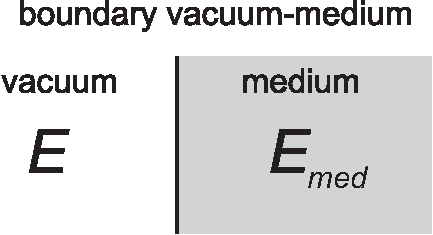
\includegraphics[width=0.48\textwidth]{wind.pdf}
\caption{Энергия частицы в вакууме $E$ не равна энергии в среде $E_{\mathrm{med}}$.}
\label{fig:1}
\end{figure}

Закон сохранения энергии сразу требует, чтобы частица в среде обладала
эффективной потенциальной энергией $V_{\mathrm{eff}}$ (подробную теорию
см.\ в~\cite{Goldberger64}). Эту энергию легко найти из соотношения
\[
E=E_{\mathrm{med}}+V_{\mathrm{eff}},
\]
то есть
\begin{equation}
V_{\mathrm{eff}}=E-E_{\mathrm{med}}
=-\frac{2\pi\hbar^2}{m\gamma}N f(E,0)=(2\pi)^3 N T(E),
\label{eq:12}
\end{equation}
где $T(E)$ --- $T$-матрица~\cite{Goldberger64} и
$f(E,0)=-(2\pi)^2\dfrac{E}{c^2\hbar^2}T(E)=-(2\pi)^2\dfrac{m\gamma}{\hbar^2}T(E)$.

Выше обсуждалась покоящаяся мишень. Но сгусток, движущийся в накопителе,
тоже можно рассматривать как мишень. Поэтому выражения~\eqref{eq:11}
и~\eqref{eq:12} следует обобщить на этот случай. Пусть $E_1$ и $\gamma_1$
--- энергия и фактор Лоренца частиц первого пучка в системе покоя
накопителя, а $E_2$ и $\gamma_2$ --- те же величины для частиц второго
пучка. Имея в виду, что фаза волны в среде лоренц-инвариантна, её можно
найти следующим образом: пусть второй пучок покоится в выбранной системе
отсчёта, тогда показатель преломления записывается в обычном виде~\eqref{eq:11}:
\begin{equation}
n_1'=1+\frac{2\pi N_2'}{(k_1')^2}f(E_1',0),
\label{eq:13}
\end{equation}
где $N_2'=\gamma_2^{-1}N_2$ --- плотность сгустка~2 в его системе покоя,
$N_2$ --- плотность второго сгустка в системе накопителя, $k_1'$ и $E_1'$
--- волновое число и энергия частиц первого сгустка в системе покоя
сгустка~2. Пусть $L$ --- длина сгустка~2 в его системе покоя, тогда
$L=\gamma_2 l$, где $l$ --- длина этого сгустка в системе накопителя.

Взаимодействие частицы из сгустка~1 (частицы~1) с частицами сгустка~2
вызывает изменение фазы волны:
\begin{equation}
\phi=k_1'(n_1'-1)L
=\frac{2\pi N_2'}{k_1'}f(E_1',0)\,L
=\frac{2\pi N_2}{k_1'}f(E_1',0)\,k_1' l.
\label{eq:14}
\end{equation}
Известно~\cite{Goldberger64}, что отношение $f(E_1',0)/k_1'$ инвариантно,
то есть $f(E_1',0)/k_1'=f(E_1,0)/k_1$, где $f(E_1,0)$ --- амплитуда
упругого когерентного рассеяния вперёд частицы~1 на движущихся частицах
сгустка~2 в системе покоя накопителя.

В результате
\begin{equation}
\phi=\frac{2\pi N_2}{k_1}f(E_1,0)\cdot l
=\frac{2\pi N_2}{k_1}f(E_1,0)\cdot v_{\mathrm{rel}}\cdot t,
\label{eq:15}
\end{equation}
где $v_{\mathrm{rel}}$ --- скорость относительного движения частицы~1
и сгустка~2 (для встречного движения
$v_{\mathrm{rel}}=(v_1+v_2)\bigl(1+v_1 v_2/c^2\bigr)^{-1}$),
а $t$ --- время взаимодействия частицы~1 со сгустком~2 в системе покоя
накопителя.

Частица со скоростью $v_1=\hbar k_1 c^2/E_1$ за время $t$ проходит
расстояние $z=v_1\cdot t$. Заметим, что расстояние $z$ отличается
от длины сгустка~2, потому что сгусток движется. Выражение~\eqref{eq:15}
можно переписать как
\begin{equation}
\phi=\frac{2\pi N_2}{k_1}f(E_1,0)\frac{v_{\mathrm{rel}}}{v_1}z
=k_1(n_1-1)z,
\label{eq:16}
\end{equation}
где показатель преломления частицы~1 пучком движущихся частиц~2 равен
\begin{equation}
n_1=1+\frac{2\pi N_2}{k_1^2}\frac{v_{\mathrm{rel}}}{v_1}f(E_1,0).
\label{eq:17}
\end{equation}
При $v_2=0$ выражение~\eqref{eq:17} переходит в обычное~\eqref{eq:11}.

Таким образом, эффективную потенциальную энергию $V_{\mathrm{eff}}$,
приобретаемую частицей~1 при столкновении с частицами сгустка~2,
можно записать как
\begin{equation}
\begin{aligned}
V_{\mathrm{eff}}
&=E_1-E_{1\,\mathrm{med}}
=E_1-\sqrt{p_1^2 c^2 n_1^2+m_1^2 c^4}\\
&=-2\pi\hbar^2 N_2 v_{\mathrm{rel}}\frac{f(E_1,0)}{p_1}
=-2\pi\hbar^2 N_2 v_{\mathrm{rel}}\frac{f(E_1',0)}{p_1'}.
\end{aligned}
\label{eq:18}
\end{equation}
Поэтому
\begin{equation}
V_{\mathrm{eff}}
=-\frac{2\pi\hbar^2 N_2}{m_1\gamma_1\gamma_2}f(E_1',0)
=(2\pi)^3 N_2 T(E_1'),
\label{eq:19}
\end{equation}
где $E_1'=m_1 c^2\gamma_1\gamma_2$ --- энергия частицы~1 в системе покоя
сгустка~2, $p_1$ --- импульс частицы~1 в системе накопителя, а $p_1'$ ---
импульс частицы~1 в системе покоя сгустка~2
($p_1'=E_1' v_1'/c^2$) и $v_1'=v_{\mathrm{rel}}$.
При получении~\eqref{eq:18} использовалось $|n_1-1|\ll 1$.

Рассмотрим теперь частицу с ненулевым спином. В этом случае амплитуда
рассеяния на нулевой угол зависит от спина частицы и, как следствие,
показатель преломления зависит от спина и может быть записан как
\begin{equation}
\hat{n}_1=1+\frac{2\pi N_2}{k_1^2}\frac{v_{\mathrm{rel}}}{v_1}\hat{f}(E_1,0),
\label{eq:20}
\end{equation}
где $\hat{f}(E_1,0)=\Tr\hat{\rho}_J\hat{F}(0)$ --- оператор амплитуды
рассеяния вперёд, действующий в объединённом спиновом пространстве
частицы и спина рассеивателя, $\hat{\rho}_J$ --- спиновая матрица
плотности рассеивателей.

Согласно изложенному выше (см.~\eqref{eq:12} и~\eqref{eq:19}), частица
в веществе обладает некоторой эффективной потенциальной энергией
$V_{\mathrm{eff}}$. Если амплитуда $\hat{f}(0)$ рассеяния частицы зависит
от спина частицы, то эффективная энергия зависит от ориентации
спина~\cite{Bary83a,Bary83b,BaryDub89,BaryShekht96,Bary92,Bary93,Bary98,BarySTORI05}:
\begin{equation}
\hat{V}_{\mathrm{eff}}
=-\frac{2\pi\hbar^2 N_2}{m_1\gamma_1\gamma_2}\hat{f}(E_1',0).
\label{eq:21}
\end{equation}
Например, амплитуда рассеяния $\hat{f}(0)$ частицы со спином $S=1$
(например, дейтрона) даже в неполяризованной мишени зависит от спина
частицы и может быть записана как
\begin{equation}
\hat{f}(E_1',0)=d+d_1\bigl(\hvec{S}\cdot\vec{e}\bigr)^2,
\label{eq:22}
\end{equation}
где $\hvec{S}$ --- оператор спина дейтрона, $\vec{e}$ --- единичный вектор
вдоль импульса дейтрона $\vec{k}$.

Подставляя выражение для $\hat{f}(0)$~\eqref{eq:22} в~\eqref{eq:21},
для частицы со спином $S=1$ получаем
\begin{equation}
\hat{V}_{\mathrm{eff}}
=-\frac{2\pi\hbar^2}{m_1\gamma_1\gamma_2}N_2\bigl(d+d_1(\hvec{S}\cdot\vec{e})^2\bigr).
\label{eq:23}
\end{equation}
Пусть ось квантования $z$ направлена вдоль $\vec{e}$, а $M$ обозначает
магнитное квантовое число. Тогда для частицы в собственном состоянии
оператора проекции спина на ось $z$, $\hat{S}_z$, эффективную
потенциальную энергию можно записать как
\begin{equation}
\hat{V}_{\mathrm{eff}}
=-\frac{2\pi\hbar^2}{m_1\gamma_1\gamma_2}N_2(d+d_1 M^2).
\label{eq:24}
\end{equation}
Согласно~\eqref{eq:24}, расщепление уровней энергии дейтрона в веществе
аналогично расщеплению атомных уровней в электрическом поле за счёт
квадратичного эффекта Штарка. Поэтому указанный эффект можно рассматривать
как вызванный расщеплением спиновых уровней частицы в псевдоэлектрическом
ядерном поле вещества.

Выражения~\eqref{eq:23} и~\eqref{eq:8} подобны; поэтому спин частицы
с $S\geqslant 1$, проходящей через неполяризованное вещество, вращается
и осциллирует (эффект двулучепреломления)~\cite{Bary92,Bary93} из-за
взаимодействия с псевдоэлектрическим ядерным полем вещества.
В дальнейшем для выражения~\eqref{eq:23} будет использоваться обозначение
$\hat{V}_E^{\mathrm{nucl}}=\hat{V}_{\mathrm{eff}}$.

\section{Вращение спина протона (дейтрона, антипротона) в накопителе
с поляризованной мишенью}

Рассмотрим теперь эксперименты, в которых используются поляризованные
пучки и мишени. В этом случае амплитуда упругого когерентного рассеяния
на нулевой угол зависит от векторной поляризации $\vec{P}_t$ ядер мишени
(если спин ядер мишени $J\geqslant 1$, появляется также добавка,
зависящая от тензорной поляризации мишени; эта добавка ниже опускается,
а общий случай рассмотрен в~\cite{Bary83a,Bary93}).

Для определённости предположим, что мишень покоится ($\gamma_2=1$,
$\gamma_1=\gamma$).

Вклад в амплитуду $\hat{f}(0)$, зависящий от векторной поляризации ядер
мишени, можно записать как
\begin{equation}
\hat{f}(\vec{P}_t,0)=A_1(\hvec{S}\cdot\vec{P}_t)+A_2(\hvec{S}\cdot\vec{e})(\vec{e}\cdot\vec{P}_t),
\label{eq:25}
\end{equation}
где $\hvec{S}$ --- оператор спина частицы. Вклады слабых $P$,$T$-нечётных
взаимодействий (см.~\cite{Bary83a,BaryShirvel05,Bary0504064,BaryGurin05})
здесь опущены.

Соответственно вклад в эффективную потенциальную энергию взаимодействия
частицы с веществом, вызванный поляризацией ядер мишени, имеет вид
\begin{equation}
\hat{V}_{\mathrm{eff}}(\vec{P}_t)
=-\frac{2\pi\hbar^2}{m\gamma}N\bigl(
A_1(\hvec{S}\cdot\vec{P}_t)+A_2(\hvec{S}\cdot\vec{e})(\vec{e}\cdot\vec{P}_t)
\bigr).
\label{eq:26}
\end{equation}
Выражение~\eqref{eq:26} можно переписать как
\begin{equation}
\hat{V}_G^{\mathrm{nucl}}
\equiv\hat{V}_{\mathrm{eff}}(\vec{P}_t)
=-(\vec{\mu}\cdot\vec{G})
=-\frac{\mu}{S}(\hvec{S}\cdot\vec{G}),
\label{eq:27}
\end{equation}
где $\mu$ --- магнитный момент частицы,
\begin{equation}
\vec{G}=\frac{2\pi\hbar^2 S}{m\gamma\mu}N\bigl(
A_1\vec{P}_t+A_2\vec{e}(\vec{e}\cdot\vec{P}_t)
\bigr).
\label{eq:28}
\end{equation}
Напомним, что энергия взаимодействия магнитного момента $\vec{\mu}$
с магнитным полем $\vec{B}$ равна
\begin{equation}
V_{\mathrm{mag}}=-(\vec{\mu}\cdot\vec{B})=-\frac{\mu}{S}(\hvec{S}\cdot\vec{B}).
\label{eq:29}
\end{equation}
Выражения~\eqref{eq:27} и~\eqref{eq:29} тождественны. Поэтому $\vec{G}$
можно интерпретировать как эффективное псевдомагнитное поле, действующее
на спин частицы в веществе с поляризованными ядрами и возникающее из-за
ядерного взаимодействия падающих частиц с рассеивателями. Подобно
прецессии спина частицы во внешнем магнитном поле, спин прецессирует
и в поле $\vec{G}$. Это явление получило название ядерной прецессии
спина частицы и впервые было описано для медленных нейтронов
в~\cite{BaryPod64} и наблюдалось в~\cite{Abragam72,Forte73,Abragam82}.

Таким образом, когда поляризованная ядерная мишень помещена внутрь
накопителя, спин частиц, проходящих через мишень, дополнительно вращается
под действием ядерного псевдомагнитного поля. Возникает вопрос, влияет ли
псевдомагнитное ядерное поле на импульс частицы подобно силам
Штерна--Герлаха. Известно, что силы Штерна--Герлаха слишком слабы,
чтобы влиять на движение частиц в накопителе~\cite{Jackson76,Derbenev73,Hoffstaetter06,Hoffstaetter00,Heinemann01},
то есть их не следует включать в уравнения движения частиц.
Псевдомагнитное ядерное поле газовой мишени много слабее внешних
магнитных полей накопителя; поэтому псевдомагнитный аналог сил
Штерна--Герлаха также не следует включать в уравнения движения частиц.
Существенно лишь действие псевдомагнитного поля на движение спина.

\section{Уравнения, описывающие движение спина частицы в накопителе}

\subsection{Взаимодействия, дающие вклад в движение спина частицы
в накопителе}

Согласно изложенному анализу, при рассмотрении движения спина частицы
в накопителе следует учитывать несколько взаимодействий:
\begin{enumerate}
\item взаимодействие магнитного и электрического дипольных моментов
с электромагнитными полями;
\item взаимодействие частицы с электрическими полями за счёт тензорной
электрической поляризуемости;
\item взаимодействие частицы с магнитными полями за счёт тензорной
магнитной поляризуемости;
\item взаимодействие частицы с псевдоэлектрическим ядерным полем вещества;
\item взаимодействие частицы с псевдомагнитным ядерным полем
поляризованного вещества.
\end{enumerate}

Уравнение для спиновой волновой функции частицы, включающее все эти
взаимодействия, имеет вид
\begin{equation}
i\hbar\frac{\partial\Psi(t)}{\partial t}
=\bigl(
\hat{H}_0+\hat{V}_{\mathrm{EDM}}+\hat{V}_{\vec{E}}+\hat{V}_{\vec{B}}
+\hat{V}_E^{\mathrm{nucl}}+\hat{V}_G^{\mathrm{nucl}}
\bigr)\Psi(t),
\label{eq:30}
\end{equation}
где $\Psi(t)$ --- спиновая волновая функция частицы; $\hat{H}_0$ ---
гамильтониан, описывающий движение спина, вызванное взаимодействием
магнитного момента с электромагнитным полем (уравнение~\eqref{eq:30}
с единственным слагаемым $\hat{H}_0$ переходит в уравнение
Томаса--Баргманна--Мишеля--Телегди); $\hat{V}_{\mathrm{EDM}}$ описывает
взаимодействие ЭДМ частицы $d$ с электрическим полем; $\hat{V}_{\vec{E}}$
описывает взаимодействие частицы с электрическим полем за счёт тензорной
электрической поляризуемости; $\hat{V}_{\vec{B}}$ --- энергия взаимодействия
частицы с магнитным полем за счёт тензорной магнитной поляризуемости;
$\hat{V}_E^{\mathrm{nucl}}$ описывает эффективную потенциальную энергию
взаимодействия частицы с псевдоэлектрическим полем мишени~\eqref{eq:23};
$\hat{V}_G^{\mathrm{nucl}}$ описывает эффективную потенциальную энергию
взаимодействия частицы с псевдомагнитным полем мишени~\eqref{eq:27}.

\subsection{Вращение спина дейтрона в электромагнитных полях накопителя}

Рассмотрим дейтрон, движущийся в накопителе без мишеней внутри, и предположим,
что давление остаточного газа мало ($10^{-10}$~Торр). В этом случае эффекты,
вызванные взаимодействиями $\hat{V}_E^{\mathrm{nucl}}$ и
$\hat{V}_G^{\mathrm{nucl}}$, можно опустить. Согласно изложенному анализу
движение спина дейтрона тем не менее нельзя описать уравнением
Томаса--Баргманна--Мишеля--Телегди: следует учитывать взаимодействия
$\hat{V}_{\vec{E}}$ и $\hat{V}_{\vec{B}}$. Соответствующие уравнения можно
записать следующим образом~\cite{BaryShirvel05,Bary0504064,BaryGurin05}:
\begin{equation}
\left\{
\begin{aligned}
\frac{d\vec{S}}{dt}
&=[\vec{S}\times\vec{\Omega}(\vec{d})]
-\frac23\frac{\alpha_T E_{\mathrm{eff}}^2}{\hbar}[\vec{e}_E\times\vec{e}_E']
-\frac23\frac{\beta_T B_{\mathrm{eff}}^2}{\hbar}[\vec{e}_B\times\vec{e}_B'],
\\[0.6em]
\frac{dP_{ik}}{dt}
&=-(\varepsilon_{jkr}P_{ij}\Omega_r(d)+\varepsilon_{jir}P_{kj}\Omega_r(d))
\\
&\quad
-\frac32\frac{\alpha_T E_{\mathrm{eff}}^2}{\hbar}
\bigl([\vec{e}_E\times\vec{S}]_i e_{E,k}+e_{E,i}[\vec{e}_E\times\vec{S}]_k\bigr)
\\
&\quad
-\frac32\frac{\beta_T B_{\mathrm{eff}}^2}{\hbar}
\bigl([\vec{e}_B\times\vec{S}]_i e_{B,k}+e_{B,i}[\vec{e}_B\times\vec{S}]_k\bigr),
\end{aligned}
\right.
\label{eq:31}
\end{equation}
где
\begin{equation*}
\begin{aligned}
\vec{\Omega}(d)&=\vec{\Omega}+\vec{\Omega}_d,\\
\vec{\Omega}
&=\frac{e}{mc}\Biggl\{
\Biggl(a+\frac{1}{\gamma}\Biggr)\vec{B}
-\Biggl(\frac{g}{2}-\frac{\gamma}{\gamma+1}\Biggr)\vec{\beta}\times\vec{E}
\Biggr\},\\
\vec{\Omega}_d
&=\frac{d}{\hbar}(\vec{E}+\vec{\beta}\times\vec{B}),\\
P_{ik}&=\Tr\rho\,\hat{Q}_{ik},\qquad
\hat{Q}_{ik}=\frac32\Biggl(S_i S_k+S_k S_i-\frac43\delta_{ik}\Biggr),
\end{aligned}
\end{equation*}
$\rho$ --- спиновая матрица плотности частицы, $m$ --- масса частицы,
$e$ --- её заряд, $P_{ik}$ --- тензор поляризации спина
($P_{xx}+P_{yy}+P_{zz}=0$), $\gamma$ --- фактор Лоренца,
$\vec{\beta}=\vec{v}/c$, $\vec{v}$ --- скорость частицы, $a=(g-2)/2$
($g$ --- гиромагнитное отношение), $\vec{E}$ и $\vec{B}$ --- электрическое
и магнитное поля в точке нахождения частицы,
$\vec{E}_{\mathrm{eff}}=(\vec{E}+\vec{\beta}\times\vec{B})$,
$\vec{B}_{\mathrm{eff}}=(\vec{B}-\vec{\beta}\times\vec{E})$,
$\vec{e}_E=(\vec{E}+\vec{\beta}\times\vec{B})/|\vec{E}+\vec{\beta}\times\vec{B}|$,
$\vec{e}_B=(\vec{B}-\vec{\beta}\times\vec{E})/|\vec{B}-\vec{\beta}\times\vec{E}|$,
$e'_{E,i}=P_{ik}e_{E,k}$, $e'_{B,i}=P_{il}e_{B,l}$, а $\Omega_r(d)$ ---
компоненты вектора $\vec{\Omega}(d)$ ($r=1,2,3$ соответствуют $x,y,z$).

\begin{figure}[htbp]
\centering
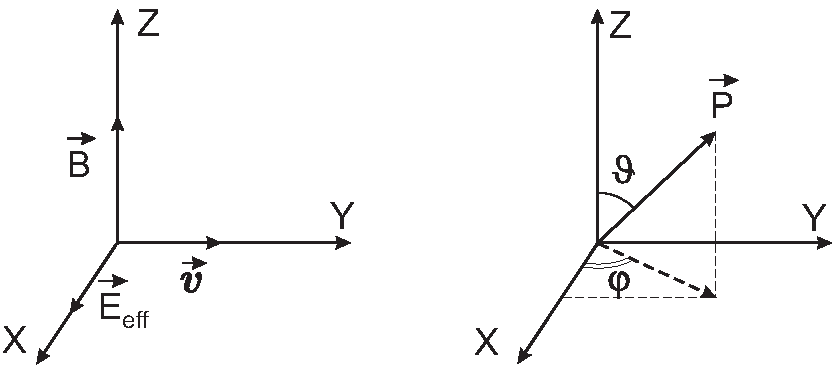
\includegraphics[width=0.62\textwidth]{coordinate.pdf}
\caption{Система координат и векторы $\vec{v}$, $\vec{E}$, $\vec{B}$.
Оси $x$, $y$, $z$ обозначаются индексами $1$, $2$, $3$.}
\label{fig:2}
\end{figure}

Уравнения движения спина~\eqref{eq:31} можно переписать как
\begin{equation}
\begin{aligned}
\frac{d\vec{S}}{dt}
&=[\vec{S}\times\vec{\Omega}(d)]
+\Omega_t[\vec{e}_E\times\vec{e}_E']
+\Omega_t^{\mu}[\vec{e}_B\times\vec{e}_B'],
\\[0.4em]
\frac{dP_{ik}}{dt}
&=-(\varepsilon_{jkr}P_{ij}\Omega_r(d)+\varepsilon_{jir}P_{kj}\Omega_r(d))
+\Omega_t'\bigl([\vec{e}_E\times\vec{S}]_i e_{E,k}+e_{E,i}[\vec{e}_E\times\vec{S}]_k\bigr)
\\
&\quad
+\Omega_t^{\prime\mu}\bigl([\vec{e}_B\times\vec{S}]_i e_{B,k}+e_{B,i}[\vec{e}_B\times\vec{S}]_k\bigr),
\end{aligned}
\label{eq:32}
\end{equation}
где
\begin{equation*}
\begin{aligned}
\Omega_t&=-\frac23\frac{\alpha_T E_{\mathrm{eff}}^2}{\hbar},\qquad
\Omega_t'=-\frac32\frac{\alpha_T E_{\mathrm{eff}}^2}{\hbar},\qquad
\Omega_t'=-\frac23\Omega_t,\\
\Omega_t^{\mu}&=-\frac23\frac{\beta_T B_{\mathrm{eff}}^2}{\hbar},\qquad
\Omega_t^{\prime\mu}=-\frac32\frac{\beta_T B_{\mathrm{eff}}^2}{\hbar},\qquad
\Omega_t^{\prime\mu}=-\frac23\Omega_t^{\mu}.
\end{aligned}
\end{equation*}
(Третьи равенства в каждой строке приведены так, как в оригинале.)

Предположим, что внешнее электрическое поле в накопителе $\vec{E}=0$
и частица движется по круговой орбите.

Рассмотрим теперь уравнение~\eqref{eq:32} в системе координат, вращающейся
с частотой вращения скорости частицы. В такой системе спин вращается
относительно импульса с частотой, определяемой $(g-2)$. Система координат
и векторы $\vec{v}$, $\vec{E}$, $\vec{B}$ показаны на рис.~\ref{fig:2}.
Оси $x$, $y$, $z$ обозначаются индексами $1$, $2$, $3$. В результате
систему~\eqref{eq:31} можно записать как
\begin{equation}
\begin{aligned}
\frac{dS_1}{dt}&=\Omega S_2-\Omega_t^{\mu} P_{23},\\
\frac{dS_2}{dt}&=-\Omega S_1+(\Omega_t^{\mu}-\Omega_t)P_{13}+\omega_d S_3,\\
\frac{dS_3}{dt}&=\Omega_t P_{12}-\omega_d S_2,
\end{aligned}
\label{eq:33}
\end{equation}
где $\omega_d=d E_{\mathrm{eff},1}/\hbar$,
\begin{equation}
\begin{aligned}
\frac{dP_{11}}{dt}&=2\Omega P_{12}+2\omega_d P_{23},\\
\frac{dP_{22}}{dt}&=-2\Omega P_{12},\\
\frac{dP_{33}}{dt}&=-2\omega_d P_{23},
\end{aligned}
\label{eq:34}
\end{equation}
\begin{equation}
\begin{aligned}
\frac{dP_{12}}{dt}&=-\Omega(P_{11}-P_{22})-\Omega_t' S_3+\omega_d P_{13},\\
\frac{dP_{13}}{dt}&=\Omega P_{23}+\Omega_t' S_2-\Omega_t^{\prime\mu} S_2-\omega_d P_{12},\\
\frac{dP_{23}}{dt}&=-\Omega P_{13}+\Omega_t^{\prime\mu} S_1-\omega_d(P_{22}-P_{33}).
\end{aligned}
\label{eq:35}
\end{equation}
Напомним, что $P_{11}+P_{22}+P_{33}=0$ и $P_{ik}=P_{ki}$.

\subsection{Вклад ЭДМ и тензорных поляризуемостей в осцилляции спина дейтрона}

Рассмотрим систему~\eqref{eq:33}--\eqref{eq:35} внимательнее.

Предположим, что у дейтрона нет ни ЭДМ, ни тензорных поляризуемостей:
тогда система~\eqref{eq:33}--\eqref{eq:35} принимает вид
\begin{equation}
\frac{dS_1}{dt}=\Omega S_2,\qquad
\frac{dS_2}{dt}=-\Omega S_1,\qquad
\frac{dS_3}{dt}=0,
\label{eq:36}
\end{equation}
\begin{equation}
\frac{dP_{11}}{dt}=2\Omega P_{12},\qquad
\frac{dP_{22}}{dt}=-2\Omega P_{12},\qquad
\frac{dP_{33}}{dt}=0,
\label{eq:37}
\end{equation}
\begin{equation}
\frac{dP_{12}}{dt}=-\Omega(P_{11}-P_{22}),\qquad
\frac{dP_{13}}{dt}=\Omega P_{23},\qquad
\frac{dP_{23}}{dt}=-\Omega P_{13}.
\label{eq:38}
\end{equation}
Это обычная система уравнений T-BMT, описывающая вращение спина частицы
с частотой $(g-2)$-прецессии $\Omega=eaB/(mc)$. Компонента $S_3$ векторной
поляризации в этих условиях постоянна ($\mathrm{d}S_3/\mathrm{d}t=0$),
как и компонента $P_{33}$ тензорной поляризации
($\mathrm{d}P_{33}/\mathrm{d}t=0$).

Предположим, что ЭДМ дейтрона отличен от нуля. Тогда система уравнений
переходит в
\begin{equation}
\frac{dS_1}{dt}=\Omega S_2,\qquad
\frac{dS_2}{dt}=-\Omega S_1+\omega_d S_3,\qquad
\frac{dS_3}{dt}=-\omega_d S_2,
\label{eq:39}
\end{equation}
\begin{equation}
\frac{dP_{11}}{dt}=2\Omega P_{12}+2\omega_d P_{23},\qquad
\frac{dP_{22}}{dt}=-2\Omega P_{12},\qquad
\frac{dP_{33}}{dt}=-2\omega_d P_{23},
\label{eq:40}
\end{equation}
\begin{equation}
\begin{aligned}
\frac{dP_{12}}{dt}&=-\Omega(P_{11}-P_{22})+\omega_d P_{13},\\
\frac{dP_{13}}{dt}&=\Omega P_{23}-\omega_d P_{12},\\
\frac{dP_{23}}{dt}&=-\Omega P_{13}-\omega_d(P_{22}-P_{33}).
\end{aligned}
\label{eq:41}
\end{equation}
Из~\eqref{eq:39}--\eqref{eq:41} следует, что наличие ненулевого ЭДМ
заставляет вертикальную компоненту $S_3$ векторной поляризации осциллировать
с частотой $(g-2)$-прецессии $\Omega$.

Согласно идее~\cite{Orlov05}, эти осцилляции можно устранить модуляцией
скорости дейтронного пучка с частотой $\Omega$:
\begin{equation}
v=v_0+\delta v\sin(\Omega t+\varphi_f).
\label{eq:42}
\end{equation}
Здесь $\varphi_f$ --- фаза вынужденных осцилляций скорости.

Поскольку $E_{\mathrm{eff}}$ зависит от $\vec{\beta}=\vec{v}/c$, она тоже
оказывается промодулированной:
\begin{equation}
E_{\mathrm{eff}}=E_{\mathrm{eff}}^0+\delta E_{\mathrm{eff}}\sin(\Omega t+\varphi_f).
\label{eq:43}
\end{equation}
Поэтому $\omega_d=d E_{\mathrm{eff}}/\hbar$ тоже модулируется с той же
частотой. Это делает произведение $\omega_d S_2\sim\sin^2(\Omega t+\varphi_f)$.
Из~\eqref{eq:39} следует
\begin{equation}
\begin{aligned}
S_3(t)
&=S_3(0)-\int_0^t\omega_d(t')S_2(t')\,\mathrm{d}t'\\
&=S_3(0)+\mathrm{const}\Biggl(
\frac{t}{2}-\frac{1}{4\Omega}\bigl(\sin(2\Omega t+2\varphi_f)-\sin 2\varphi_f\bigr)
\Biggr).
\end{aligned}
\label{eq:44}
\end{equation}
Согласно~\eqref{eq:44}, компонента $S_3(t)$ содержит как линейно растущий
член, так и член, осциллирующий с частотой $\Omega$ и имеющий малую амплитуду.
Для лучших условий измерения важно сделать $S_3(0)=0$, то есть спин частицы
изначально должен лежать в горизонтальной плоскости. Именно поэтому спин
частицы выбирают лежащим в горизонтальной плоскости.

Аналогичные рассуждения показывают, что $P_{33}(t)$ тоже содержит линейно
растущую компоненту. Однако когда спин лежит в горизонтальной плоскости,
$P_{33}(0)\ne 0$.

Важно отметить, что при ориентации спина, удовлетворяющей условию
$\cos^2\vartheta=1/3$
($\cos\vartheta=\sqrt{1/3}$, $\sin\vartheta=\sqrt{2/3}$),
получается компонента $P_{33}(0)=0$, тогда как $S_3(0)\ne 0$.
Поэтому, выбирая $\vartheta$, удовлетворяющий условию
$\cos\vartheta=\sqrt{1/3}$, можно использовать компоненту $P_{33}$
и для измерений ЭДМ.

Рассмотрим теперь вклад электрической и магнитной тензорных поляризуемостей.
Тогда вместо системы~\eqref{eq:39}--\eqref{eq:41} следует рассматривать
систему~\eqref{eq:33}--\eqref{eq:35}.

Из~\eqref{eq:33}--\eqref{eq:35} следуют некоторые интересные следствия.
Как уже упоминалось, в экспериментах по поиску ЭДМ планируется измерять
рост вертикальной компоненты $S_3$.

Согласно~\eqref{eq:33}, зависимость $S_3$ от времени описывается уравнением
\begin{equation}
\frac{dS_3}{dt}=\Omega_t P_{12}-\omega_d S_2
\label{eq:45}
\end{equation}
и определяется как ЭДМ, так и тензорной поляризуемостью дейтрона.
Интересно, что производная компоненты тензорной поляризации $P_{33}$
не содержит вклада тензорной электрической поляризуемости и пропорциональна
только ЭДМ:
\begin{equation}
\frac{dP_{33}}{dt}=-2\omega_d P_{23}.
\label{eq:46}
\end{equation}
Поэтому важно измерять и компоненту $P_{33}$. Согласно изложенному,
ориентация спина для этого случая определяется условием
$\cos^2\vartheta=1/3$.

\subsection{Вклад тензорной магнитной поляризуемости в осцилляции спина дейтрона}

Вклады ЭДМ и поляризуемостей во вращение и осцилляции спина малы.
Поэтому их можно рассматривать как возмущения полной системы~\eqref{eq:33}--\eqref{eq:35}
и изучать роль каждого отдельно.

Система уравнений с учётом вклада тензорной магнитной поляризуемости
$\beta_T$ имеет вид
\begin{equation}
\begin{aligned}
\frac{dS_1}{dt}&=\Omega S_2-\Omega_t^{\mu} P_{23},\\
\frac{dS_2}{dt}&=-\Omega S_1+\Omega_t^{\mu} P_{13},\\
\frac{dP_{13}}{dt}&=\Omega P_{23}-\Omega_t^{\prime\mu} S_2,\\
\frac{dP_{23}}{dt}&=-\Omega P_{13}+\Omega_t^{\prime\mu} S_1.
\end{aligned}
\label{eq:47}
\end{equation}
Вводя новые переменные $S_+=S_1+i S_2$ и $G_+=P_{13}+i P_{23}$
и перегруппировывая уравнения~\eqref{eq:47} для $S_+$ и $G_+$, получаем
\begin{equation}
\frac{dS_+}{dt}=-i\Omega S_++i\Omega_t^{\mu} G_+,\qquad
\frac{dG_+}{dt}=-i\Omega G_++i\Omega_t^{\prime\mu} S_+.
\label{eq:48}
\end{equation}
Будем искать $S_+\sim\tilde{S}_+ e^{-i\omega t}$,
$G_+\sim\tilde{G}_+ e^{-i\omega t}$; тогда~\eqref{eq:48} переходит в
\begin{equation}
\omega\tilde{S}_+=\Omega\tilde{S}_+-\Omega_t^{\mu}\tilde{G}_+,\qquad
\omega\tilde{G}_+=\Omega\tilde{G}_+-\Omega_t^{\prime\mu}\tilde{S}_+.
\label{eq:49}
\end{equation}
Решение этой системы легко находится в виде
\begin{equation}
(\omega-\Omega)^2-\Omega_t^{\mu}\Omega_t^{\prime\mu}=0,
\label{eq:50}
\end{equation}
что в итоге даёт
\begin{equation}
\omega_{1,2}=\Omega\pm\sqrt{\Omega_t^{\mu}\Omega_t^{\prime\mu}}.
\label{eq:51}
\end{equation}
Решение~\eqref{eq:48} можно записать как
\begin{equation}
S_+(t)=c_1 e^{-i\omega_1 t}+c_2 e^{-i\omega_2 t}
=|c_1|e^{-i(\omega_1 t-\delta_1)}+|c_2|e^{-i(\omega_2 t-\delta_2)}.
\label{eq:52}
\end{equation}
Поэтому
\begin{equation}
S_1(t)=|c_1|\cos(\omega_1 t-\delta_1)+|c_2|\cos(\omega_2 t-\delta_2),
\label{eq:53}
\end{equation}
\begin{equation}
S_2(t)=-|c_1|\sin(\omega_1 t-\delta_1)-|c_2|\sin(\omega_2 t-\delta_2).
\label{eq:54}
\end{equation}
Согласно~\eqref{eq:53} и~\eqref{eq:54}, ненулевая тензорная магнитная
поляризуемость дейтрона заставляет спин вращаться с двумя частотами
$\omega_1$ и $\omega_2$ вместо $\Omega$. Разность частот
\[
\Delta\omega=\omega_1-\omega_2
=2\sqrt{\Omega_t^{\mu}\Omega_t^{\prime\mu}}
=\frac{\beta_T B_{\mathrm{eff}}^2}{\hbar}.
\]

Напомним теперь, что взаимодействие ЭДМ с электрическим полем заставляет
спин дейтрона вращаться вокруг направления этого поля и приводит
к появлению компоненты $S_3$, пропорциональной $S_2(t)$:
\begin{equation}
\frac{dS_3}{dt}\sim -\omega_d S_2.
\label{eq:55}
\end{equation}
Поэтому
\begin{equation}
\frac{dS_3}{dt}
=\omega_d\bigl(|c_1|\sin(\omega_1 t-\delta_1)+|c_2|\sin(\omega_2 t-\delta_2)\bigr).
\label{eq:56}
\end{equation}
Согласно идее~\cite{Orlov05}, для измерения ЭДМ следует модулировать
скорость частицы ($v=v_0+\delta v\sin(\Omega_f t+\varphi_f)$) с частотой
$\Omega_f$, близкой к частоте $\Omega$ $(g-2)$-прецессии.

Если предположить, что магнитная поляризуемость равна нулю, то
$\omega_1=\omega_2=\Omega$ и спин вращается в горизонтальной плоскости
с частотой $\Omega$. В этом случае модуляция скорости с той же частотой
$\Omega_f=\Omega$ даёт
\begin{equation}
\frac{dS_3}{dt}\sim\sin^2(\Omega t),
\label{eq:57}
\end{equation}
и вертикальную компоненту можно записать как
\[
S_3=\int_0^t\frac{dS_3}{dt'}\,\mathrm{d}t'
\sim\int_0^t\sin^2\Omega t'\,\mathrm{d}t'
\sim\frac12\Biggl(t-\frac{1}{2\Omega}\sin\Omega t\Biggr).
\]
Вертикальная компонента, очевидно, включает член, линейно растущий со временем,
и член малой амплитуды, осциллирующий с высокой частотой.

Однако $\omega_1\ne\omega_2$, и модуляция скорости, например, с частотой
$\Omega=\omega_1$ даёт медленную осцилляцию спина с частотой
$(\omega_1-\omega_2)$ вместо линейного роста.

Согласно оценке~\cite{Chen98}, тензорная магнитная поляризуемость
$\beta_T\sim 2\times 10^{-40}$; поэтому в поле $B\sim 10^{4}$~Гс частота
биений $\Delta\omega\sim 10^{-5}$. Измерение частоты биений позволяет
найти тензорную магнитную поляризуемость дейтрона (или ядра).

Таким образом, из-за наличия тензорной магнитной поляризуемости
горизонтальная компонента спина вращается вокруг $\vec{B}$ с двумя
частотами $\omega_1$, $\omega_2$ вместо ожидаемого вращения с частотой
$\Omega$. Поэтому компонента $S_3$ испытывает осцилляции, подобные
вызываемым ЭДМ. Следовательно, модуляция скорости частицы с частотой
$\Omega$ устраняет осцилляции с этой частотой, но осцилляции $S_3$
с частотой $\Delta\omega$ остаются (аналогично $P_{33}$). Изучение
этих осцилляций необходимо, поскольку они могут исказить измерения ЭДМ.

\subsection{Вклад тензорной электрической поляризуемости в осцилляции
спина дейтрона}

Рассмотрим теперь вклад, вызванный тензорной электрической поляризуемостью.
Из системы~\eqref{eq:34} следует
\begin{equation}
\frac{d(P_{11}-P_{22})}{dt}=4\Omega P_{12},
\label{eq:58}
\end{equation}
\begin{equation}
\frac{d^2 P_{12}}{dt^2}
=-\Omega\frac{d(P_{11}-P_{22})}{dt}-\Omega_t'\frac{dS_3}{dt}
=-(4\Omega^2+\Omega_t\Omega_t')P_{12}.
\label{eq:58b}
\end{equation}
Таким образом, имеем уравнение
\begin{equation}
\frac{d^2 P_{12}}{dt^2}+\omega_{12}^2 P_{12}=0,
\label{eq:59}
\end{equation}
где $\omega_{12}=\sqrt{4\Omega^2+\Omega_t\Omega_t'}\approx 2\Omega$,
поскольку $\Omega_t\Omega_t'\ll\Omega^2$.

Решение этого уравнения можно искать в виде
\begin{equation}
P_{12}=c_1\cos\omega_{12}t+c_2\sin\omega_{12}t.
\label{eq:60}
\end{equation}
Найдём коэффициенты $c_1$ и $c_2$: при $t=0$ уравнение~\eqref{eq:60}
даёт $c_1=P_{12}(0)$. Коэффициент $c_2$ находится из
\begin{equation}
\Biggl.\frac{dP_{12}}{dt}\Biggr|_{t\to 0}=\omega_{12}c_2.
\label{eq:61}
\end{equation}
Поэтому
\begin{equation}
c_2=\frac{1}{\omega_{12}}\Biggl.\frac{dP_{12}}{dt}\Biggr|_{t\to 0}.
\label{eq:62}
\end{equation}
Из уравнения~\eqref{eq:35}
\begin{equation}
\Biggl.\frac{dP_{12}}{dt}\Biggr|_{t\to 0}
=-\Omega\bigl(P_{11}|_{t\to 0}-P_{22}|_{t\to 0}\bigr)
\label{eq:63}
\end{equation}
следует, что
\begin{equation}
c_2=-\frac{P_{11}-P_{22}}{2}
\label{eq:64}
\end{equation}
и
\begin{equation}
P_{12}=P_{12}(0)\cos\omega_{12}t-\frac{P_{11}-P_{22}}{2}\sin\omega_{12}t.
\label{eq:65}
\end{equation}
В результате для вертикальной компоненты спина $S_3$ можно записать
уравнение
\begin{equation}
\frac{dS_3}{dt}
=\Omega_t P_{12}(t)
=\Omega_t\Biggl[
P_{12}(0)\cos 2\Omega t
-\frac{P_{11}(0)-P_{22}(0)}{2}\sin 2\Omega t
\Biggr].
\label{eq:66}
\end{equation}
Как видно, вертикальная компонента спина осциллирует с частотой $2\Omega$.

Уравнение, описывающее вклад в $S_3$ тензорной электрической поляризуемости
и ЭДМ, имеет вид~\eqref{eq:33}:
\begin{equation}
\frac{dS_3}{dt}=\Omega_t P_{12}-\omega_d S_2.
\label{eq:67}
\end{equation}
Поскольку частота осцилляций $S_2$ равна $\Omega$, произведение
$\omega_d S_2$ содержит неосциллирующие члены (см.\ раздел~5.3).
В результате вклад в $S_3$, вызванный ЭДМ, либо линейно растёт со временем,
когда $\Omega_f=\Omega$, либо медленно осциллирует с частотой
$\Omega_f-\Omega$, когда $\Omega_f\ne\Omega$.

Важно, что модуляция скорости $v=v_0+\delta v\sin(\Omega_f t+\varphi_f)$
приводит к осцилляции $E_{\mathrm{eff}}$ (см.~\eqref{eq:43}) и, следовательно,
$E_{\mathrm{eff}}^2$ тоже осциллирует со временем и оказывается
пропорциональной $\sin^2(\Omega_f t+\varphi_f)$. В результате вклад в $S_3$,
вызванный тензорной электрической поляризуемостью, можно записать как
\begin{equation}
\frac{dS_3(\alpha_T)}{dt}
\sim\Delta\Omega_t\sin^2(\Omega_f t+\varphi_f)
\Biggl[
P_{12}(0)\cos 2\Omega t
-\frac{P_{11}(0)-P_{22}(0)}{2}\sin 2\Omega t
\Biggr],
\label{eq:68}
\end{equation}
где $\Delta\Omega_t=-\dfrac23\dfrac{\alpha_T}{\hbar}(\delta E_{\mathrm{eff}})^2$,
то есть
\begin{equation}
\frac{dS_3(\alpha_T)}{dt}
\sim -\frac12\Delta\Omega_t\cos(2\Omega_f t+2\varphi_f)
\Biggl[
P_{12}(0)\cos 2\Omega t
-\frac{P_{11}(0)-P_{22}(0)}{2}\sin 2\Omega t
\Biggr].
\label{eq:69}
\end{equation}
Согласно~\eqref{eq:69}, для частично поляризованного дейтронного пучка
производная $\mathrm{d}S_3/\mathrm{d}t$ зависит от компонент поляризации
дейтрона $P_{12}$ и $(P_{11}(0)-P_{22})/2$.

Для простоты рассмотрим дейтронный пучок в чистом поляризационном состоянии.
В этом случае компоненты $P_{12}$ и $(P_{11}(0)-P_{22})/2$ можно вычислить,
используя явное выражение для спиновых волновых функций. Пусть
$\vec{e}(\vartheta,\varphi)$ --- единичный вектор вдоль спина дейтрона
($\vartheta$ и $\varphi$ --- полярный и азимутальный углы,
см.\ рис.~\ref{fig:2}). Тогда спиновую волновую функцию, описывающую
состояние спина дейтрона с магнитным квантовым числом $m=1$, можно
записать следующим образом (в декартовом базисе):
\begin{equation}
\chi_1(\vartheta,\varphi)
=\begin{pmatrix}a_x\\ a_y\\ a_z\end{pmatrix}
=-\frac{1}{\sqrt{2}}
\begin{pmatrix}
\cos\vartheta\cos\varphi-i\sin\varphi\\
\cos\vartheta\sin\varphi+i\cos\varphi\\
-\sin\vartheta
\end{pmatrix}.
\label{eq:70}
\end{equation}
Вектор поляризации можно записать как
\begin{equation}
\vec{S}=\langle\hvec{S}\rangle=\chi_1^+\hvec{S}\chi_1=i[\vec{a}\times\vec{a}^*]
\label{eq:71}
\end{equation}
и компоненты тензора поляризации
\begin{equation}
\langle P_{ik}\rangle
=\chi_1^+\hat{Q}_{ik}\chi_1
=-\frac32\Biggl\{a_i a_k^*+a_k a_i^*-\frac23\Biggr\},
\label{eq:72}
\end{equation}
где $\hat{Q}_{ik}$ --- спиновый тензор ранга~2
($\hat{Q}_{ik}=\dfrac12(\hat{S}_i\hat{S}_k+\hat{S}_k\hat{S}_i-\dfrac43\delta_{ik}S)$).
Поэтому
\begin{equation}
P_{12}=\frac34\sin 2\varphi\sin^2\vartheta,
\label{eq:73}
\end{equation}
\begin{equation}
\frac{P_{11}-P_{22}}{2}=\frac34\cos 2\varphi\sin^2\vartheta,
\label{eq:74}
\end{equation}
\begin{equation}
P_{33}=-\frac32\Biggl(\sin^2\vartheta-\frac23\Biggr).
\label{eq:75}
\end{equation}
Используя~\eqref{eq:69}, \eqref{eq:73}, \eqref{eq:74}, получаем
\begin{equation}
\frac{dS_3(\alpha_T)}{dt}
\sim -\frac38\Delta\Omega_t\sin^2\vartheta\cos(2\Omega_f t+2\varphi_f)
[\sin 2\varphi\cos 2\Omega t-\cos 2\varphi\sin 2\Omega t].
\label{eq:76}
\end{equation}
Из~\eqref{eq:76} следует, что $\mathrm{d}S_3/\mathrm{d}t$ медленно
осциллирует с частотой $(\Omega_f-\Omega)$.

В идеальном случае, когда $\Omega_f=\Omega$ (как предлагается
в~\cite{Orlov05} для измерения ЭДМ), \eqref{eq:76} переходит в
\begin{equation}
\frac{dS_3(\alpha_T)}{dt}
=-\frac38\Delta\Omega_t\sin^2\vartheta\cos(2\Omega t+2\varphi_f)\sin(2\Omega t-2\varphi).
\label{eq:77}
\end{equation}
В общем случае, когда фазы $\varphi_f$ и $\varphi$ произвольны,
\eqref{eq:77} содержит члены, не зависящие от времени, и поэтому $S_3$
линейно растёт со временем, как сигнал от ЭДМ.

Интересно, что выбирая $\varphi_f=-\varphi$, получаем
\begin{equation}
\frac{dS_3(\alpha_T)}{dt}
\sim\cos(2\Omega t-2\varphi)\sin(2\Omega t-2\varphi)
=\frac12\sin(4\Omega t-4\varphi),
\label{eq:78}
\end{equation}
что делает этот вклад в $S_3$ быстро осциллирующим и подавленным.
Но даже в этом идеальном случае (хотя в реальной ситуации
$\Omega\ne\Omega_f$) остаётся вклад, вызванный тензорной магнитной
поляризуемостью~\eqref{eq:9}.

Измерение этих вкладов позволяет найти тензорную электрическую
поляризуемость. Согласно оценкам~\cite{Chen98},
$\alpha_T\sim 10^{-40}$~см$^3$, поэтому для поля
$E_{\mathrm{eff}}=B\sim 10^{4}$~Гс частота
$\Omega_t\sim 10^{-5}$~с$^{-1}$. При рассмотрении модуляции можно оценить
$\Delta\Omega_t\sim\Omega_t(\delta v/v_0)^2$; тогда, полагая
$(\delta v/v_0)^2\sim 10^{-2}$--$10^{-3}$, получаем
$\Delta\Omega_t\sim 10^{-7}$--$10^{-8}$~с$^{-1}$, что превышает величину
$\omega_d$ для ЭДМ дейтрона $d=10^{-29}\,e\,\mathrm{cm}$.

\section{Вращение спина частицы в накопителе с внутренней мишенью}

Пусть теперь внутри накопителя помещена газовая мишень. Согласно
разделу~5.1, на движение спина в этом случае также влияют ядерные
псевдоэлектрическое и псевдомагнитное поля.

Описание движения спина усложняется, потому что многократное рассеяние
в мишени изменяет как угловой разброс, так и деполяризацию пучка частиц
и должно быть учтено.

Поэтому для вывода уравнений эволюции спина частицы следует использовать
формализм спиновой матрицы плотности.

Матрица плотности системы <<дейтрон+мишень>> есть
\begin{equation}
\rho=\rho_p\otimes\rho_t,
\label{eq:79}
\end{equation}
где $\rho_p$ --- матрица плотности пучка частиц, $\rho_t$ --- матрица
плотности мишени.

Уравнение для матрицы плотности частицы можно записать как~\cite{BaryShekht96,BaryShirvel05}
\begin{equation}
\frac{d\rho_p}{dt}
=-\frac{i}{\hbar}[\hat{H}_p,\rho_p]
+\Biggl(\frac{\partial\rho_p}{\partial t}\Biggr)_{\mathrm{col}},
\label{eq:80}
\end{equation}
где $\hat{H}_p$ --- гамильтониан, описывающий движение частицы во внешних
электромагнитных полях, а $(\partial\rho_p/\partial t)_{\mathrm{col}}$
описывает эволюцию матрицы плотности из-за столкновений с атомами (ядрами)
мишени.

Столкновительный член можно записать следующим образом:
\begin{equation}
\begin{aligned}
\Biggl(\frac{\partial\rho_p}{\partial t}\Biggr)_{\mathrm{col}}
&=v N\,\Tr_t\Biggl\{
\frac{2\pi i}{k}\bigl[F(\theta=0)\rho-\rho F^+(\theta=0)\bigr]
\\
&\qquad\qquad
+\int\mathrm{d}\Omega\, F(\vec{k}')\rho(\vec{k}')F^+(\vec{k}')
\Biggr\},
\end{aligned}
\label{eq:81}
\end{equation}
где $\vec{k}'=\vec{k}+\vec{q}$, вектор $\vec{q}$ --- импульс, переданный
ядру вещества падающей частицей, $v$ --- скорость падающих частиц,
$N$ --- плотность атомов в веществе, $F$ --- амплитуда рассеяния,
зависящая от спиновых операторов дейтрона и ядра (атома) вещества,
$F^+$ --- эрмитово сопряжение оператора $F$. Первый член в~\eqref{eq:81}
описывает когерентное упругое рассеяние частицы на ядрах вещества,
второй --- многократное рассеяние. Рассмотрим первый член в~\eqref{eq:81}.
Его можно записать как
\begin{equation}
\Biggl(\frac{\partial\rho_p}{\partial t}\Biggr)_{\mathrm{col}}^{(1)}
=v N\frac{2\pi i}{k}\bigl[\hat{f}(0)\rho_p-\rho_p\hat{f}(0)^+\bigr].
\label{eq:83}
\end{equation}
Амплитуда $\hat{f}(0)$ рассеяния частицы в мишени на нулевой угол равна
\begin{equation}
\hat{f}(0)=\Tr_t\hat{F}(0)\rho_t.
\label{eq:84}
\end{equation}
В результате получаем
\begin{equation}
\Biggl(\frac{\partial\rho_p}{\partial t}\Biggr)_{\mathrm{col}}^{(1)}
=-\frac{i}{\hbar}\bigl(\hat{V}_{\mathrm{eff}}\rho_p-\rho_p\hat{V}_{\mathrm{eff}}^+\bigr),
\label{eq:85}
\end{equation}
где
\begin{equation}
\begin{aligned}
\hat{V}_{\mathrm{eff}}
&=-\frac{2\pi\hbar^2}{m\gamma}N\hat{f}(0)\\
&=-\frac{2\pi\hbar^2}{m\gamma}N\bigl(
d+A_1(\hvec{S}\cdot\vec{P}_t)+A_2(\hvec{S}\cdot\vec{e})(\vec{e}\cdot\vec{P}_t)
+d_1(\hvec{S}\cdot\vec{e})^2
\bigr).
\end{aligned}
\label{eq:86}
\end{equation}
Последнее выражение можно переписать как
\begin{equation}
\hat{V}_{\mathrm{eff}}
=-\frac{2\pi\hbar^2}{m\gamma}N d
-\frac{\mu}{S}(\vec{S}\cdot\vec{G})
-\frac{2\pi\hbar^2}{m\gamma}N d_1(\hvec{S}\cdot\vec{e})^2,
\label{eq:87}
\end{equation}
где $\vec{G}=\dfrac{2\pi\hbar^2 S}{m\gamma\mu}N\bigl(A_1\vec{P}_t+A_2\vec{e}(\vec{e}\cdot\vec{P}_t)\bigr)$;
см.~\eqref{eq:28}. Для частиц со спином $1/2$ член, пропорциональный $d_1$,
отсутствует.

Окончательно выражение~\eqref{eq:80} принимает вид
\begin{equation}
\begin{aligned}
\frac{d\rho_p}{dt}
&=-\frac{i}{\hbar}[\hat{H}_p,\rho_p]
-\frac{i}{\hbar}\bigl(\hat{V}_{\mathrm{eff}}\rho_p-\rho_p\hat{V}_{\mathrm{eff}}^+\bigr)
\\
&\quad
+v N\,\Tr_t\int\mathrm{d}\Omega\, F(\vec{k}')\rho(\vec{k}')F^+(\vec{k}').
\end{aligned}
\label{eq:88}
\end{equation}
Последний член в этой формуле, пропорциональный $\Tr_t$, описывает
процесс многократного рассеяния и вызванную им деполяризацию спина.

При изучении взаимодействия частиц с мишенью внутри накопителя плотность
мишени выбирается так, чтобы многократное рассеяние в ней за время
наблюдения было мало; деполяризация пучка тоже оказывается малой.

Для частиц высоких энергий существенно рассеяние на малые углы. Поэтому
большая часть рассеянных частиц остаётся на своих орбитах. Для этого
случая последний член следует учитывать.

Дальнейший анализ уравнений~\eqref{eq:88} в настоящей работе проводится
для такого времени эксперимента, которое позволяет отбросить последний
член в~\eqref{eq:88}.

В результате имеем
\begin{equation}
\frac{d\rho_p}{dt}
=-\frac{i}{\hbar}[\hat{H}_p,\rho_p]
-\frac{i}{\hbar}\bigl(\hat{V}_{\mathrm{eff}}\rho_p-\rho_p\hat{V}_{\mathrm{eff}}^+\bigr).
\label{eq:89}
\end{equation}

Теперь можно получить уравнение, описывающее эволюцию спиновых свойств
частицы в накопителе. Вектор поляризации имеет вид
\begin{equation}
\vec{P}
=\frac{\Tr\rho_p(t)\,(\hvec{S}/S)}{\Tr\rho_p(t)}
=\frac{\Tr\rho_p(t)\,\hvec{S}}{I(t)\,S},
\label{eq:90}
\end{equation}
где $I(t)=\Tr\rho_p(t)$ --- интенсивность пучка.

Из~\eqref{eq:90} можно получить дифференциальное уравнение, позволяющее
найти поляризацию пучка:
\begin{equation}
\frac{d\vec{P}}{dt}
=\frac{\Tr\bigl(\mathrm{d}\rho_p(t)/\mathrm{d}t\bigr)\,\hvec{S}}{S I(t)}
-\vec{P}\frac{1}{I(t)}\frac{dI(t)}{dt}.
\label{eq:91}
\end{equation}
Когда спин частицы $S=1$, следует также найти тензор поляризации:
\begin{equation}
P_{ik}=\frac{\Tr\rho_p\hat{Q}_{ik}}{I(t)}.
\label{eq:92}
\end{equation}
Изменение тензорной поляризации со временем можно записать как
\begin{equation}
\frac{dP_{ik}}{dt}
=\frac{1}{I(t)}\Tr\Biggl(\frac{d\rho_p}{dt}\hat{Q}_{ik}\Biggr)
-P_{ik}\frac{1}{I(t)}\frac{dI(t)}{dt},
\label{eq:93}
\end{equation}
$\hat{Q}_{ik}=\dfrac32\bigl(S_i S_k+S_k S_i-\dfrac43\delta_{ik}\bigr)$.
Используя уравнение для матрицы плотности~\eqref{eq:88} и
выражения~\eqref{eq:91}, \eqref{eq:93}, можно получить уравнение для
случая, когда на движение спина влияют псевдоэлектрическое и
псевдомагнитное ядерные поля.

Рассмотрим сначала частицы со спином $S=1/2$. Матрицу плотности такой
частицы можно записать как
\begin{equation}
\rho_{p\,1/2}=I_{1/2}(t)\Biggl(\frac12\hat{I}+(\vec{P}\cdot\hvec{S})\Biggr),
\label{eq:94}
\end{equation}
где $\hat{I}$ --- единичная матрица в спиновом пространстве, $\hvec{S}$ ---
оператор спина.

С помощью~\eqref{eq:90} можно найти, что
\begin{equation}
\begin{aligned}
\frac{d I_{1/2}(t)}{dt}
&=-\frac{i}{\hbar}\Tr\bigl(
\hat{V}_{\mathrm{eff}}\rho_{p\,1/2}-\rho_{p\,1/2}\hat{V}_{\mathrm{eff}}^+
\bigr)
=-\Biggl(\varkappa+\frac{2\mu}{\hbar}(\vec{G}_2\cdot\vec{P})\Biggr)I_{1/2}(t),
\end{aligned}
\label{eq:95}
\end{equation}
где $\varkappa=v N\sigma_{\mathrm{tot}}$, $v$ --- скорость частицы,
$\sigma_{\mathrm{tot}}$ --- полное сечение рассеяния частицы на
неполяризованном ядре, $\vec{G}_2$ --- мнимая часть псевдомагнитного
ядерного поля.

Выражение~\eqref{eq:95} можно переписать как
\begin{equation}
\frac{d I_{1/2}(t)}{dt}=-\varkappa_{\mathrm{abs}}(\vec{P})\,I_{1/2}(t),
\label{eq:96}
\end{equation}
где коэффициент поглощения
\[
\varkappa_{\mathrm{abs}}
=v N\Biggl[
\sigma_{\mathrm{tot}}+\frac12\sigma_1(\vec{P}\cdot\vec{P}_t)
+\frac12\sigma_2(\vec{P}\cdot\vec{e})(\vec{e}\cdot\vec{P}_t)
\Biggr]
=\varkappa+\vec{P}\cdot\vec{g}_t
\]
и $\vec{g}_t=\dfrac12 v N(\sigma_1\vec{P}_t+\sigma_2\vec{e}(\vec{e}\cdot\vec{P}_t))$.

Сечение $\sigma_1=\sigma_{\mathrm{tot}}^{\uparrow\uparrow}(\vec{e}\perp\vec{P}_t)
-\sigma_{\mathrm{tot}}^{\uparrow\downarrow}(\vec{e}\perp\vec{P}_t)$ ---
разность сечений рассеяния частицы на поляризованном ядре при $\vec{P}$,
параллельном ($\vec{P}\uparrow\uparrow\vec{P}_t$) и антипараллельном
($\vec{P}\uparrow\downarrow\vec{P}_t$) вектору поляризации мишени
$\vec{P}_t$, в условиях, когда импульс частицы ортогонален вектору
поляризации мишени ($\vec{e}\perp\vec{P}_t$).

Сечение $\sigma_2=\sigma_{\mathrm{tot}}^{\uparrow\uparrow}(\vec{e}\parallel\vec{P}_t)
-\sigma_{\mathrm{tot}}^{\uparrow\downarrow}(\vec{e}\parallel\vec{P}_t)$ ---
разность сечений рассеяния частицы на поляризованном ядре при $\vec{P}$,
параллельном и антипараллельном $\vec{P}_t$, в условиях, когда импульс
частицы параллелен вектору поляризации мишени ($\vec{e}\parallel\vec{P}_t$).

Уравнение~\eqref{eq:96} описывает хорошо известный факт: коэффициент
поглощения пучка частиц в поляризованной мишени зависит от взаимной
ориентации векторов поляризации пучка и мишени.

Получим теперь уравнение, описывающее эволюцию векторной поляризации
частицы под действием псевдомагнитного ядерного поля $\vec{G}$.

Согласно~\eqref{eq:90}, \eqref{eq:91} можно получить
\begin{equation}
\begin{aligned}
\frac{d\vec{P}}{dt}
&=\frac{1}{S I_{1/2}(t)}\Tr\frac{d\rho_p}{dt}\,\hvec{S}
-\vec{P}\frac{1}{I_{1/2}(t)}\frac{d I_{1/2}(t)}{dt}\\
&=-\frac{2\mu}{\hbar}[\vec{G}_1\times\vec{P}]
-\frac{2\mu}{\hbar}\bigl(\vec{G}_2-\vec{P}(\vec{G}_2\cdot\vec{P})\bigr),
\end{aligned}
\label{eq:97}
\end{equation}
где $\vec{G}_1=\Reop\vec{G}$, $\vec{G}_2=\Imop\vec{G}$.

Уравнение~\eqref{eq:97} можно переписать как
\begin{equation}
\frac{d\vec{P}}{dt}
=[\vec{P}\times\vec{\Omega}_{\mathrm{nuc}}]
-(\vec{g}_t-\vec{P}(\vec{P}\cdot\vec{g}_t)),
\label{eq:98}
\end{equation}
где $\vec{\Omega}_{\mathrm{nuc}}$ --- частота прецессии спина
в псевдомагнитном ядерном поле
\begin{equation}
\vec{\Omega}_{\mathrm{nuc}}
=\frac{2\mu}{\hbar}\vec{G}_1
=\frac{2\pi\hbar}{m\gamma}N\bigl(
\Reop A_1\,\vec{P}_t+\Reop A_2\,\vec{e}(\vec{e}\cdot\vec{P}_t)
\bigr).
\label{eq:99}
\end{equation}
Добавляя вклад псевдомагнитного ядерного поля~\eqref{eq:98}
к уравнению T-BMT~\eqref{eq:32}, получаем уравнение, описывающее
эволюцию спина частицы, движущейся в накопителе с поляризованной
мишенью внутри:
\begin{equation}
\frac{d\vec{P}}{dt}
=\bigl[\vec{P}\times\bigl(\vec{\Omega}(d)+\vec{\Omega}_{\mathrm{nuc}}\bigr)\bigr]
-(\vec{g}_t-\vec{P}(\vec{P}\cdot\vec{g}_t)),
\label{eq:100}
\end{equation}
\begin{equation}
\frac{d I_{1/2}(t)}{dt}
=-(\varkappa+(\vec{P}\cdot\vec{g}_t))I_{1/2}(t),
\label{eq:101}
\end{equation}
где $\vec{g}_t=\dfrac12 v N(\sigma_1\vec{P}_t+\sigma_2\vec{e}(\vec{e}\cdot\vec{P}_t))$.

Напомним, что уравнение~\eqref{eq:100}, подобно уравнению T-BMT, описывает
вектор поляризации частицы, движущейся по определённой траектории.
Строго говоря, чтобы найти вектор поляризации пучка частиц, движущегося
в накопителе, $\vec{P}$ следует усреднить по распределению частиц
в фазовом пространстве пучка~\cite{Jackson76,Derbenev73,Hoffstaetter06,Hoffstaetter00,Heinemann01,Mane05}.

Вклад псевдомагнитного ядерного поля в движение спина частицы с $S=1$
(например, дейтрона) можно получить аналогичным образом. Спиновая матрица
плотности для частицы со спином~1 записывается как
\begin{equation}
\rho_1=I_1(t)\Biggl(
\frac13\hat{I}+\frac12(\vec{P}\cdot\hvec{S})+\frac19 P_{ik}\hat{Q}_{ik}
\Biggr).
\label{eq:102}
\end{equation}
Эффективная потенциальная энергия взаимодействия дейтрона с поляризованной
мишенью выражается как
\[
\hat{V}_{\mathrm{eff}}
=-\frac{2\pi\hbar^2}{m\gamma}N d
-\frac{\mu}{S}(\hvec{S}\cdot\vec{G})
-\frac{2\pi\hbar^2}{m\gamma}N d_1(\hvec{S}\cdot\vec{e})^2
\]
(см.~\eqref{eq:87}).

Энергия $\hat{V}_{\mathrm{eff}}$ для дейтрона (в отличие от частицы
со спином $S=1/2$) содержит как взаимодействие дейтрона с псевдомагнитным
полем, так и с псевдоэлектрическим полем (член, пропорциональный $d_1$).
Уравнения, описывающие вращение спина дейтрона (эффект двулучепреломления)
в псевдоэлектрическом поле неполяризованной внутренней мишени накопителя,
получены в~\cite{BaryShirvel05}.

Если внутренняя мишень в накопителе поляризована, то, используя~\eqref{eq:87},
\eqref{eq:89} и~\eqref{eq:102}, можно найти изменение интенсивности пучка
и вектора поляризации:
\begin{equation}
\frac{d I_1(t)}{dt}
=-\Biggl[
(\varkappa+2(\vec{g}_t\cdot\vec{P}))
-\frac{\chi}{3}(2+P_{ik}e_i e_k)
\Biggr]I_1(t),
\label{eq:103}
\end{equation}
где $\chi=-4\pi v N/k\,\Imop d_1=-v N(\sigma_{M=1}-\sigma_{M=0})$,
$\varkappa=v N\sigma_{M=0}$, $\sigma_{M=1}$ и $\sigma_{M=0}$ --- полные
сечения рассеяния дейтрона на неполяризованном ядре для состояния дейтрона
с магнитным квантовым числом $M=1$ и $M=0$ соответственно (ось квантования
направлена вдоль $\vec{e}$).

Вектор поляризации можно записать как
\begin{equation}
\begin{aligned}
\frac{d\vec{P}}{dt}
&=[\vec{P}\times\vec{\Omega}_{\mathrm{nuc}}]
-\frac23 P_{ik}g_{t,k}-\frac43\vec{g}_t+2\vec{P}(\vec{P}\cdot\vec{g}_t)
+\frac{\eta}{3}[\vec{e}\times\vec{e}']
\\
&\quad
+\frac{\chi}{2}\bigl(\vec{e}(\vec{e}\cdot\vec{P})+\vec{P}\bigr)
-\frac{2\chi}{3}\vec{P}
-\frac{\chi}{3}(\vec{e}\cdot\vec{e}')\vec{P},
\end{aligned}
\label{eq:104}
\end{equation}
где $\eta=-4\pi N/k\,\Reop d_1$ и $e'_i=P_{ik}e_k$.

Согласно~\eqref{eq:104}, ядерное псевдомагнитное поле вызывает прецессию
спина дейтрона с частотой $\vec{\Omega}_{\mathrm{nuc}}$. Вклад~\eqref{eq:104}
следует добавить к уравнению~\eqref{eq:32}, чтобы они описывали движение
спина дейтрона в накопителе с мишенью внутри.

Аналогичный подход позволяет описать эволюцию тензорной
поляризации~\eqref{eq:93}, но она слишком громоздка, чтобы приводить её здесь.

Однако когда поглощением пучка частиц в мишени можно пренебречь, все
изменения в уравнении, описывающем поведение спина дейтрона, сводятся
к замене $\vec{\Omega}(d)$ на новое значение
$(\vec{\Omega}(d)+\vec{\Omega}_{\mathrm{nuc}})$.

Заметим, что поскольку мишень внутри накопителя имеет конечный размер,
частица, движущаяся в накопителе, взаимодействует с мишенью лишь в отдельные
моменты времени (выражения для $\vec{\Omega}_{\mathrm{nuc}}$ и $\vec{g}_t$
содержат плотность $N$, которая означает плотность в точке нахождения
частицы, то есть $N=N(t)$). Поэтому $\vec{\Omega}_{\mathrm{nuc}}$ и
$\vec{g}_t$ осциллируют с частотой обращения частицы в накопителе
$\Omega_0$.

Для дальнейшего анализа разложим $\vec{\Omega}_{\mathrm{nuc}}$ и $\vec{g}_t$
в ряд Фурье и оставим только нулевую гармонику. В этом случае
$\vec{\Omega}_{\mathrm{nuc}}$ и $\vec{g}_t$ оказываются постоянными
и могут быть записаны как
\begin{equation}
\begin{aligned}
\vec{\Omega}_{\mathrm{nuc}}
&=\frac{2\pi\hbar}{m\gamma}N\bigl(
\Reop A_1\,\vec{P}_t+\Reop A_2\,\vec{e}(\vec{e}\cdot\vec{P}_t)
\bigr)\frac{l}{v T}
\\
&=\frac{2\pi\hbar}{m\gamma}\frac{j_t}{L}\bigl(
\Reop A_1\,\vec{P}_t+\Reop A_2\,\vec{e}(\vec{e}\cdot\vec{P}_t)
\bigr)
\\
&=\frac{2\pi\hbar}{m\gamma}\frac{j_t\nu}{v}\bigl(
\Reop A_1\,\vec{P}_t+\Reop A_2\,\vec{e}(\vec{e}\cdot\vec{P}_t)
\bigr),
\end{aligned}
\label{eq:105}
\end{equation}
где $l$ --- длина мишени, $j_t=N\cdot l$ --- плотность мишени в см$^{-2}$
(обычно для поляризованной газовой мишени $j_t\approx 10^{14}$~см$^{-2}$),
$T$ --- период обращения пучка в накопителе, $\nu$ --- частота обращения
частицы в накопителе, $L$ --- длина орбиты частицы внутри накопителя.

Нулевая гармоника для $\vec{g}_t$ имеет вид
\begin{equation}
\begin{aligned}
\vec{g}_t
&=\frac12 v N\bigl(\sigma_1\vec{P}_t+\sigma_2\vec{e}(\vec{e}\cdot\vec{P}_t)\bigr)
\frac{l}{v T}
=\frac12 j_t\nu\bigl(\sigma_1\vec{P}_t+\sigma_2\vec{e}(\vec{e}\cdot\vec{P}_t)\bigr).
\end{aligned}
\label{eq:106}
\end{equation}

Оценим теперь величину эффекта. Для протонов, антипротонов и дейтронов
с энергией от МэВ до ГэВ величина $\Reop A_1\sim 10^{-12}$--$10^{-13}$~см.
Полагая $\nu\sim 10^{6}$~с$^{-1}$, получаем для частоты ядерной прецессии
$\Omega_{\mathrm{nuc}}=10^{-4}$--$10^{-5}$~с$^{-1}$.

Заметим (см.~\eqref{eq:18} и~\eqref{eq:19}), что отношение
$\gamma^{-1}\Reop A_{1(2)}$ пропорционально $T$-матрице и, следовательно,
$\Omega_{\mathrm{nuc}}$ зависит от энергии частицы лишь из-за возможной
зависимости $T$-матрицы от энергии.

Полученная оценка для $\Omega_{\mathrm{nuc}}$ позволяет ожидать,
например для COSY, измерения угла поворота спина
$\vartheta=\Omega_{\mathrm{nuc}} t\approx 10^{-2}$--$10^{-3}$~рад
за время наблюдения $t\sim 10^{2}$~с. Эта величина вполне наблюдаема.

Чтобы прецессия спина в псевдомагнитном ядерном поле не подавлялась
магнитным полем накопителя $\vec{B}$, можно использовать либо
псевдомагнитное ядерное поле, вращающееся с частотой $(g-2)$-прецессии~\cite{BaryGurin05},
либо другие методы компенсации $(g-2)$-прецессии
(см., например,~\cite{Onderwater05,Farley04,Orlov05}).

Рассмотрим теперь конкретный пример. Пусть ось $OZ$ ортогональна
плоскости орбиты ($OZ\parallel\vec{B}$) (см.\ рис.~\ref{fig:2}).
Псевдомагнитное поле направлено вдоль оси $OX$. В этом случае для частицы
в прямолинейном промежутке накопителя вертикальная компонента спина
вращается вокруг направления псевдомагнитного поля в плоскости $ZOY$.
Следует наблюдать изменение вертикальной (или горизонтальной) компоненты спина.

Поскольку типичный угол поворота спина $\vartheta=\Omega_{\mathrm{nuc}} t\ll 1$,
зависимость вертикальной компоненты спина от времени можно записать как
\begin{equation}
S_3(t)=S_3(0)-\frac12\vartheta^2 t^2
=S_3(0)-\Omega_{\mathrm{nuc}}^2 t^2.
\label{eq:107}
\end{equation}
Эффект можно усилить, добавив магнитное поле $\vec{b}\gg\vec{G}_1$,
направленное вдоль псевдомагнитного поля $\vec{G}_1$ (вдоль оси $OX$
в рассматриваемом случае). Тогда угол поворота выражается как
$\vartheta=\vartheta_{\mathrm{mag}}+\vartheta_{\mathrm{nuc}}
=(\Omega_{\mathrm{mag}}(\vec{b})+\Omega_{\mathrm{nuc}})\cdot t$,
а вертикальная компонента
$S_3(t)=S_3(0)-\dfrac12\vartheta_{\mathrm{mag}}^2 t^2
-\vartheta_{\mathrm{mag}}\vartheta_{\mathrm{nuc}}$
(членами $\sim\vartheta_{\mathrm{nuc}}^2$ пренебрегаем).

Изменяя направление поля $\vec{b}$ в ходе эксперимента (то есть меняя
знак $\vartheta_{\mathrm{mag}}$), получаем возможность измерить разность
$S_3(\vec{b}\uparrow\uparrow\vec{G}_1,t)-S_3(\vec{b}\uparrow\downarrow\vec{G}_1,t)
=2\vartheta_{\mathrm{mag}}\vartheta_{\mathrm{nuc}}$.

Это позволяет изучить возможность наблюдения эффекта и тем самым
измерить спин-зависимую часть амплитуды упругого когерентного рассеяния
на нулевой угол.

\section{Заключение}

В настоящей работе получены уравнения, описывающие движение спина частицы
в накопителе, с учётом вкладов тензорных электрической и магнитной
поляризуемостей частицы, а также вращения спина и двулучепреломления
в поляризованном веществе газовой мишени.

Подробно рассмотрено влияние тензорных электрической и магнитной
поляризуемостей на движение спина в резонансном эксперименте по ЭДМ дейтрона.

Показано, что помимо ЭДМ электрическая и магнитная поляризуемости тоже
дают вклад в вертикальную компоненту спина $S_3$. Более того, электрическая
поляризуемость даёт вклад в компоненту $S_3$ даже тогда, когда ЭДМ дейтрона
полагается равным нулю, и тем самым может имитировать вклад ЭДМ.
Показано, что в отличие от вертикальной компоненты спина $S_3$ компонента
$P_{33}$ тензора поляризации не содержит вклада электрической
поляризуемости, тогда как вклад магнитной поляризуемости проявляется
лишь когда ЭДМ дейтрона отличен от нуля.

Также показано, что когда угол $\vartheta$ между направлением спина
и вертикальной осью удовлетворяет условию
$\sin\vartheta=\sqrt{2/3}$ ($\cos\vartheta=\sqrt{1/3}$), начальное
значение $P_{33}$ оказывается $P_{33}(0)=0$. В результате вклад ЭДМ
в измеряемый сигнал линейно растёт со временем, начиная с нуля.
Поэтому измерение компоненты $P_{33}$ тензорной поляризации дейтрона
представляет особый интерес, особенно потому, что ненулевая компонента
$P_{33}$ однозначно указывает на наличие ЭДМ (в отличие от компоненты
$S_3$, появление которой может быть вызвано тензорной электрической
поляризуемостью, а не ЭДМ).

Также показано, что изучение эффектов вращения спина и двулучепреломления
для частицы высокой энергии в накопителе позволяет измерить спин-зависимую
вещественную часть амплитуды когерентного упругого рассеяния вперёд.

\begin{thebibliography}{99}

\bibitem{Lehar}
C.~Lechanoine-Lelue and F.~Lehar, \textit{Rev.\ Mod.\ Phys.} \textbf{65} (1993) 47.

\bibitem{Engels}
R.~Engels et al., \textit{Proc.\ 6th Int.\ Conf.\ on Nuclear Physics at Storage Rings STORI'05},
\textit{Matter Mater.} \textbf{30} (2005) 381.

\bibitem{Kacharava}
A.~Kacharava, F.~Rathmann and C.~Wilkin (ANKE Collaboration),
COSY Proposal 152, preprint nucl-ex/0511028 (2005).

\bibitem{Bary83a}
V.~G.~Baryshevsky, \textit{Sov.\ J.\ Nucl.\ Phys.} \textbf{38} (1983) 569.

\bibitem{Bary83b}
V.~G.~Baryshevsky, \textit{Phys.\ Lett.\ B} \textbf{120} (1983) 267.

\bibitem{BaryDub89}
V.~G.~Baryshevsky and I.~Ya.~Dubovskaya, \textit{Phys.\ Lett.\ B} \textbf{256} (1989) 529.

\bibitem{BaryShekht96}
V.~G.~Baryshevsky and A.~G.~Shekhtman, \textit{Phys.\ Rev.\ C} \textbf{53} (1996) 267.

\bibitem{Bary92}
V.~G.~Baryshevsky, \textit{Phys.\ Lett.\ A} \textbf{171} (1992) 431.

\bibitem{Bary93}
V.~G.~Baryshevsky, \textit{J.\ Phys.\ G: Nucl.\ Part.\ Phys.} \textbf{19} (1993) 273.

\bibitem{Bary98}
V.~G.~Baryshevsky, K.~G.~Batrakov and S.~Cherkas,
\textit{J.\ Phys.\ G: Nucl.\ Part.\ Phys.} \textbf{24} (1998) 2049.

\bibitem{BarySTORI05}
V.~Baryshevsky, \textit{Proc.\ 6th Int.\ Conf.\ on Nuclear Physics at Storage Rings STORI'05},
\textit{Matter Mater.} \textbf{30} (2005) 277.

\bibitem{BaryPod64}
V.~G.~Baryshevsky and M.~I.~Podgoretsky, \textit{Zh.\ Eksp.\ Teor.\ Fiz.} \textbf{47} (1964) 1050.

\bibitem{Abragam72}
A.~Abragam et al., \textit{C.\ R.\ Acad.\ Sci.} \textbf{274} (1972) 423.

\bibitem{Forte73}
M.~Forte, \textit{Nuovo Cimento A} \textbf{18} (1973) 727.

\bibitem{Abragam82}
A.~Abragam and M.~Goldman, \textit{Nuclear Magnetism: Order and Disorder}
(Oxford: Oxford University Press, 1982).

\bibitem{Chiladze06}
D.~Chiladze et al., \textit{Phys.\ Rev.\ ST Accel.\ Beams} \textbf{9} (2006) 050101.

\bibitem{Olsen72}
G.~G.~Ohlsen, \textit{Rep.\ Prog.\ Phys.} \textbf{35} (1972) 717.

\bibitem{Onderwater05}
C.~J.~G.~Onderwater et al., \textit{Proc.\ 6th Int.\ Conf.\ on Nuclear Physics at Storage Rings STORI'05},
\textit{Matter Mater.} \textbf{30} (2005) 231.

\bibitem{Bary05hepex}
V.~Baryshevsky et al., LANL preprint hep-ex/0501045 (2005).

\bibitem{Jackson76}
J.~D.~Jackson, \textit{Rev.\ Mod.\ Phys.} \textbf{48} (1976) 427.

\bibitem{Derbenev73}
Ya.~S.~Derbenev and A.~M.~Kondratenko, \textit{Sov.\ Phys.\ JETP} \textbf{37} (1973) 968.

\bibitem{Hoffstaetter06}
G.~H.~Hoffstaetter, \textit{High Energy Polarized Proton Beams: A Modern View}
(Springer Tracts in Modern Physics vol.~218) (Berlin: Springer, 2006).

\bibitem{Hoffstaetter00}
G.~H.~Hoffstaetter, LANL preprint physics/0006007 (2000).

\bibitem{Heinemann01}
K.~Heinemann and D.~P.~Barber, \textit{Nucl.\ Instrum.\ Methods Phys.\ Res.\ A}
\textbf{463} (2001) 62; \textbf{469} (2001) 294;
K.~Heinemann and G.~H.~Hoffstaetter, \textit{Phys.\ Rev.\ E} \textbf{54} (1996) 4240.

\bibitem{Mane05}
S.~R.~Mane, Yu.~M.~Shatunov and K.~Yokoya, \textit{Rep.\ Prog.\ Phys.} \textbf{68} (2005) 1997.

\bibitem{Farley04}
F.~Farley et al., \textit{Phys.\ Rev.\ Lett.} \textbf{93} (2004) 052001.

\bibitem{Orlov05}
Yu.~Orlov, \textit{Proc.\ 6th Int.\ Conf.\ on Nuclear Physics at Storage Rings STORI'05},
\textit{Matter Mater.} \textbf{30} (2005) 223.

\bibitem{BaryShirvel05}
V.~Baryshevsky and A.~Shirvel, LANL preprint hep-ph/0503214 (2005).

\bibitem{Bary0504064}
V.~Baryshevsky, LANL preprint hep-ph/0504064 (2005).

\bibitem{BaryGurin05}
V.~Baryshevsky and A.~Gurinovich, LANL preprint hep-ph/0506135 (2005).

\bibitem{FordHirt61}
G.~W.~Ford and C.~W.~Hirt, University of Michigan Report (1961), unpublished.

\bibitem{Thomas26}
L.~H.~Thomas, \textit{Nature} \textbf{117} (1926) 514;
L.~H.~Thomas, \textit{Phil.\ Mag.} \textbf{3} (1927) 1.

\bibitem{Frenkel26}
J.~Frenkel, \textit{Z.\ Phys.} \textbf{37} (1926) 243.

\bibitem{BMT59}
V.~Bargmann, L.~Michel and V.~L.~Telegdi, \textit{Phys.\ Rev.\ Lett.} \textbf{2} (1959) 435.

\bibitem{Chen98}
Jiunn-Wei Chen, H.~W.~Grie{\ss}hammer, M.~J.~Savage and R.~P.~Springer,
\textit{Nucl.\ Phys.\ A} \textbf{644} (1998) 221; preprint nucl-th/9806080.

\bibitem{Lax51}
M.~Lax, \textit{Rev.\ Mod.\ Phys.} \textbf{23} (1951) 287.

\bibitem{Goldberger64}
M.~L.~Goldberger and K.~M.~Watson, \textit{Collision Theory} (New York: Wiley, 1964).

\end{thebibliography}

\end{document}

